\documentclass{article}
\usepackage{atma_arxiv,times}
\usepackage[T1]{fontenc}
\input{math_commands.tex}

\usepackage{microtype}
\usepackage{hyperref}
\usepackage{url}
\usepackage{booktabs}
\usepackage{amsmath}
\usepackage{amssymb}
\usepackage{amsfonts}
\usepackage{amsthm}
\usepackage{graphicx}
\usepackage{array}
\usepackage{longtable}
\usepackage{pdflscape}
\usepackage{listings}
\usepackage{placeins}
\usepackage{multirow}
\graphicspath{{./}}

\definecolor{darkblue}{rgb}{0,0,0.5}
\hypersetup{colorlinks=true,citecolor=darkblue,linkcolor=darkblue,urlcolor=darkblue}
\lstset{
  basicstyle=\scriptsize\ttfamily,
  columns=fullflexible,
  keepspaces=true,
  breaklines=true,
  frame=single,
  framerule=0.3pt,
  xleftmargin=0.5em,
  xrightmargin=0.5em,
  aboveskip=0.6em,
  belowskip=0.6em,
  showstringspaces=false
}
\newtheorem{assumption}{Assumption}
\newtheorem{proposition}{Proposition}
\newtheorem{corollary}{Corollary}

\title{ATMA: Long-Context Language Modeling via Polar Attention and Gated-Delta Compression Memory}
\author{Habibullah Akbar \\
Kreasof AI \\
Jakarta, Indonesia \\
\texttt{habibullah.akbar@kreasof.my.id}}

\iclrfinalcopy
\begin{document}
\maketitle

\begin{abstract}
What determines whether a language model extrapolates beyond its training length? We study attention--memory interactions and checkpoint variability using \textbf{ATMA}, a 378M-parameter hybrid combining Polar Attention with gated-delta recurrent memory. Polar uses a normalized direction, a bounded participation-ratio magnitude, and learned length scaling. In a complete 120-cell, 1B-token factorial, memory improves Polar's teacher-forced target-token retrieval at 64K in all 20 matched cells, by 47.8 percentage points on average. We then train matched NoPE, RoPE, and Polar models for 9.816B tokens at length 2K. The primary Polar checkpoint retains 62.7\% exact FinePDFs retrieval at 8K and 34.4\% target-token accuracy and 9.0\% exact five-token accuracy overall at 256K, with all exact successes on synthetic haystacks. Two fresh paired runs retain a retrieval advantage over NoPE but reach only 0.0\% and 3.83\% exact accuracy. A post-hoc intervention caps the most retentive head in each checkpoint: primary NoPE and Polar 256K bits per byte fall from 8.097 to 1.595 and from 1.825 to 1.501. Both NoPE replications recover the likelihood improvement; the Polar replications have no comparable gate outlier and remain essentially unchanged by the cap. A separately optimized TDA hybrid reaches 0.2\% token retrieval but 40\% adapted BABILong accuracy at 256K, exposing distinct retrieval and reasoning trade-offs. Prospective controls resolve attribution: across three matched initialization triplets, Polar strictly outperforms temperature-matched softmax on natural-text exact retrieval by an average of 22.18 percentage points, and retains a 37.18-point advantage across 30 independent documents. The one-head retention cap rescues likelihood without conferring a general retrieval boost, delineating the boundaries of retention stability.
Code: \url{https://github.com/kreasof-ai/atma}
\end{abstract}

\section{Introduction}

Large language models increasingly process code repositories, books, legal documents, and scientific papers that exceed their pretraining sequence length. Full softmax attention preserves token-level access in principle, but its probability mass can disperse as the key set grows~\citep{nakanishi2025scalable,velickovic2025softmax,barbero2024glasses}. Sliding windows bound cost by removing older tokens from direct access. Recurrent sequence models instead keep fixed-size state but compress history. Long-context modeling therefore exposes a multi-objective trade-off among retrieval fidelity, sequence likelihood, reasoning, short-context quality, and serving cost.

Two questions organize this study: how does recurrent memory interact with the attention rule, and why can checkpoints with nearly identical short-context loss extrapolate differently? In the primary comparison, Polar delays the loss of exact natural-text associative recall relative to NoPE and RoPE, but every tested model eventually reaches zero. Fresh paired runs preserve a Polar retrieval advantage while showing substantially weaker extreme-length exact recall. We report the primary checkpoints and replications separately so that architectural trends and checkpoint-specific magnitudes remain distinguishable.

We present \textbf{ATMA}, a hybrid architecture that combines short gated convolutions with four \textbf{Polar Attention} layers as global mixers. Polar Attention represents ``what matched'' with a normalized direction and ``how much matched'' with a bounded participation-ratio channel. A learned null sink follows the extreme-value scale of irrelevant scores. Each global layer also contains gated-delta memory, providing a compressed recurrent history alongside full-context attention (Appendix~\ref{appendix:theory}).

\begin{figure}[t]
\centering
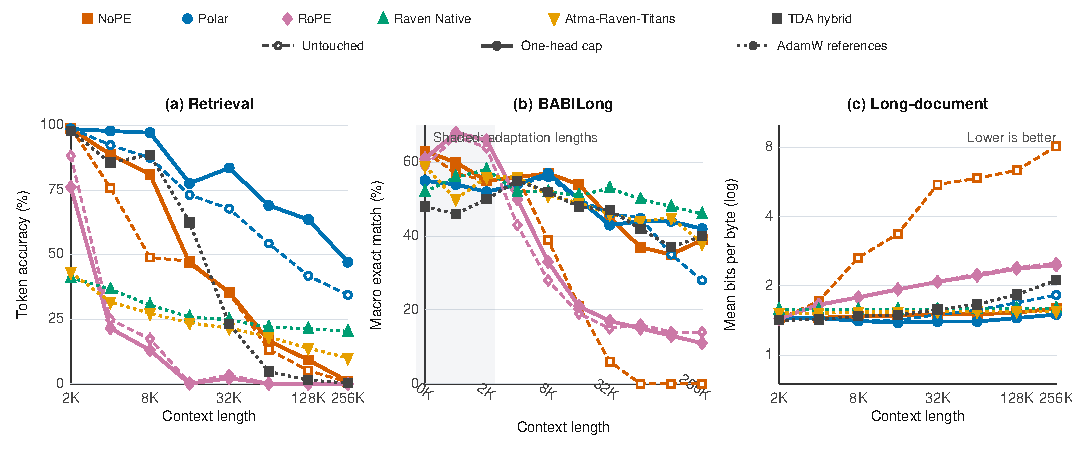
\includegraphics[width=\linewidth]{fig_main_results.pdf}
\caption{Primary checkpoints before and after the one-head retention cap. Dashed/solid curves show untouched/capped attention variants in matching colors; dotted curves show untouched Raven and TDA hybrid references. \textbf{Left:} teacher-forced target-token retrieval. \textbf{Center:} BABILong exact match after adaptation. \textbf{Right:} mean fixed-target BPB (log scale; lower is better). Table~\ref{tab:replication_main} reports the fresh runs; Section~\ref{sec:retention_audit} explains the intervention.}
\label{fig:main_results}
\end{figure}

We make three contributions. First, a complete 120-cell factorial measures how memory interacts with the attention core across regularizers, distractor alignment, and training windows. Second, matched 9.816B-token runs characterize retrieval, likelihood, reasoning, short-context quality, and serving; two fresh NoPE/Polar pairs test the retrieval and likelihood findings. Raven and TDA hybrid provide separately optimized references~\citep{raven2026,huang2026threshold}. Third, we connect checkpoint-specific likelihood collapse to isolated near-unit retention gates through a selective inference-only intervention. The NoPE likelihood repair repeats in both fresh pairs, while Polar's cap benefit does not. This localizes one extrapolation failure without establishing a general cap benefit or the training origin of the outlier.

\section{Related Work}

Softmax attention~\citep{Vaswani+2017} has quadratic compute and can lose selectivity as the number of keys grows. RoPE~\citep{rope2021} and ALiBi~\citep{alibi2021} alter positional information while retaining dense simplex normalization. Scalable-Softmax, adaptive-temperature analyses, and sparse alternatives address dispersion or length-dependent sharpness~\citep{nakanishi2025scalable,velickovic2025softmax,vasylenko2026sparse}. Threshold Differential Attention (TDA) uses a $\sqrt{\log n}$ threshold motivated by maxima of noise scores~\citep{huang2026threshold}. Polar combines length-dependent temperature and extreme-value scaling with a differentiable null sink and a bounded magnitude channel. We compare Polar with matched NoPE and RoPE controls and a separately optimized TDA hybrid (Appendix~\ref{appendix:protocol}). Comparisons with the remaining methods are conceptual.

Linear attention, state-space models, and gated recurrences exchange full-resolution token access for compressed fixed-size history~\citep{mamba2023,deltanet2024,yang2024gated,titans2025}. Near-unit gates create very long timescales and can enter saturation regimes~\citep{gu2020gating}. Stability-aware SSM parameterizations likewise distinguish stable eigenvalues from a robust distance to the stability boundary~\citep{wang2024stablessm}. Stuffed Mamba directly studies an inability-to-forget failure and post-training interventions that restore forgetting~\citep{chen2025stuffed}. Our audit asks the corresponding checkpoint-level question for the gated-delta branch used here: a sigmoid keeps each retention value below one, but does not enforce a useful uniform margin from one. Raven combines routed sparse memory, decay dynamics, and gated-delta recurrence~\citep{raven2026}. We treat it as a strong sub-quadratic baseline, but not as an attention ablation because it uses a different model family and optimizer. Hybrid models such as LFM2 combine local and global mixers for efficiency~\citep{lfm2_2025,physics_lms_2025}. ATMA follows this hybrid pattern while changing the global mixer and adding a recurrent memory stream.

\section{Method}

\subsection{Hybrid architecture}

ATMA is a 16-layer decoder whose block order repeats local--local--global--local four times, yielding 12 LFM2-style gated convolutional layers and global attention at blocks 3, 7, 11, and 15. All blocks use pre-normalization and squared-ReLU MLPs. The attention variants share hidden size 1024, eight query heads, two key-value heads, head dimension 128, tokenizer, data order, optimizer, schedule, and training budget. Only the attention core changes among NoPE, RoPE, and Polar. Canon depthwise causal convolutions are applied to $q$, $k$, and $v$ before attention~\citep{physics_lms_2025}.

\subsection{Polar attention}

For query $i$ and its $n_i=i+1$ visible keys, let $\sigma_{ij}=q_i^\top k_j/\sqrt{d_k}$, broadcasting the two KV heads to the eight query heads. Each head learns a length temperature and a virtual null logit,
\begin{equation}
 t_i=1+\operatorname{softplus}(\alpha)\log n_i,\qquad
 \nu_i=b+\operatorname{softplus}(\gamma)\sqrt{\log(n_i+1)}.
\label{eq:length}
\end{equation}
The second term tracks the extreme-value scale of unrelated scores. Appending the null as a softmax competitor gives
\begin{equation}
 w_i=\operatorname{softmax}\!\left(t_i[\sigma_{i\bullet},\nu_i]\right),\qquad
 s_i=\sum_jw_{ij}v_j+w_{iN}v_{\rm null}.
\end{equation}
The \emph{direction} channel is $c_i=s_i/\max(\lVert s_i\rVert_2,\varepsilon)$, hence $\lVert c_i\rVert_2\leq1$. To retain bounded information about match multiplicity, real-key weights are renormalized as $\hat w_{ij}=w_{ij}/\sum_kw_{ik}$ and summarized by the participation ratio
\begin{equation}
 n_{{\rm eff},i}=\left(\sum_j\hat w_{ij}^2\right)^{-1},\quad
 m_{{\rm eff},i}=n_{{\rm eff},i}(1-w_{iN}),\quad
 \mu_i=\tanh\!\left(\operatorname{softplus}(\beta)\log(1+m_{{\rm eff},i})\right).
\end{equation}
Thus $\mu_i\in[0,1)$, while the direction channel removes radial scale. This is a channel decomposition, not an independence claim, because changing the match set can rotate $c_i$. The Polar output is $y_i^{\rm polar}=W_o(c_i\odot\sigma(W_{\rm gate}c_i))+W_\mu\mu_i$, combining gated direction with learned magnitude. Pre-integration tests rejected simpler choices. Additive soft counts leaked with length, fixed or relative floors were overtaken by noise tails, and an unbounded $\log m$ channel left the training range. The standalone prototype was not retained. Appendix~\ref{appendix:polar_implementation} separates this design history from the reproducible integrated oracle and kernel tests. The promoted recipe disables the distractor-alignment loss tested in the factorial.

\subsection{Gated-delta memory}

Each global layer also maintains a per-head recurrent state $M_t\in\mathbb{R}^{d_v\times d_k}$. With unit-normalized keys and queries ($k_t\leftarrow k_t/\lVert k_t\rVert_2$, $q_t\leftarrow q_t/\lVert q_t\rVert_2$), write gate $\beta_t=\sigma(W_\beta x_t+b_\beta)$, and retention $\gamma_t=\sigma(W_\gamma x_t+b_\gamma+b_{\rm init})$ with $b_{\rm init}=+3.9$, the decay-first, self-inclusive recurrence is
\begin{equation}
 M_t=\gamma_tM_{t-1}(I-\beta_tk_tk_t^\top)+\beta_tv_tk_t^\top,\qquad r_t=M_tq_t.
\label{eq:memory}
\end{equation}
RMS-normalized $r_t$ is gated via $g_t=\sigma(W_g x_t+b_g)$, projected with zero-initialized $W_{\rm mem}$, and added to $y_t^{\rm polar}$. Unit $L_2$ normalization keeps update eigenvalues along $k$ within the gate-controlled range; unnormalized or RMS-normalized keys caused delta recurrence to diverge. Under bounded values and a uniformly contractive retention gate, Appendix~\ref{appendix:theory} gives a sequence-length-independent state bound. The sigmoid guarantees $0<\gamma_t<1$ pointwise, but not the fixed margin $\gamma_t\leq\bar\gamma<1$ assumed by that result. The implied half-life $H_{1/2}=\log(1/2)/\log\gamma$ diverges as $\gamma\rightarrow1$. Section~\ref{sec:retention_audit} audits this distinction empirically.

Figure~\ref{fig:machinery} summarizes the two mechanisms and their controlled diagnostics. Appendix~\ref{appendix:reg_modes} defines every regularization mode in the factorial sweep, Appendix~\ref{appendix:polar_implementation} gives the numerical oracle and streaming Triton implementation, and Appendix~\ref{appendix:systems} details the kernel and serving optimizations.

\begin{figure}[t]
\centering
\includegraphics[width=0.88\linewidth]{fig_machinery.pdf}
\caption{Controlled ATMA diagnostics. \textbf{Left:} the effective match count maps to a bounded magnitude channel. \textbf{Right:} the tested gated-delta state stays flat with length, unlike an ungated Hebbian memory. These diagnostics illustrate the mechanism but do not prove network-level stability.}
\label{fig:machinery}
\end{figure}

\section{Experimental Design}

\subsection{Recipe selection}
Stage I trains all $3\times5\times2\times2\times2=120$ combinations of attention type (Polar, RoPE, NoPE), regularization, distractor loss, memory, and a 1024-token training window. Every model receives about 1B FineWeb-Edu tokens at length 2048 on an NVIDIA L4, and every evaluation uses full context. These are distinct factorial cells, not seed replicates. Stage I selects the promoted recipe and is not used for headline absolute comparisons.

\subsection{Matched comparison}
Stage II trains 378.16--378.22M-parameter NoPE, RoPE, and Polar models for 9.816B tokens at length 2048 in the same L40S software and hardware environment. All three use the same Muon/AdamW parameter split. Raven Native (388.54M) and Atma-Raven-Titans (382.37M) use the same data, tokenizer, token budget, and device class, but use AdamW. In a 1B-token Raven Native pilot with the ATMA Muon schedule, validation loss improved to 3.76 nats at step 625, then became unstable and ended at 4.62. Retrieval remained at 0\% through 64K. We therefore report the stable Raven models as a separate model-family/optimizer group. The single failed pilot does not establish incompatibility with every Muon configuration. A 388.64M-parameter TDA hybrid adds the same 9.816B-token, 2K budget with AdamW and microbatch four; it is a recipe-level reference, not an isolated attention substitution.

\paragraph{Evaluation.}
The primary retrieval grid has 28,800 model--trial evaluations across six models (4,800 per model): passkey/NIAH, synthetic/FinePDFs haystacks, eight lengths from 2K to 256K, three depths, and 50 trials per cell. Cues and digit targets are paired across lengths, depths, and models; all real-text trials reuse prefixes of one concatenated FinePDFs stream. We score five teacher-forced target tokens and exact five-token matches, rather than instruction-following generation. Fixed-target BPB scores one 256-token span in each of 18 documents (8 FinePDFs, 5 PG-19, 5 Proof-Pile), totaling 4,608 target tokens per model and length. Additional evaluations cover BABILong adaptation and greedy exact match~\citep{babilong2024}, eight 2K tasks (22,939 examples per model), and single-sequence serving on one L40S. BABILong has ten held-out rows per task and length with custom splits and prompts. These are controlled diagnostics with limited independent text coverage; Appendix~\ref{appendix:protocol} gives aggregation and pairing details.

\section{Results}

\subsection{Component selection}

Table~\ref{tab:ablation} summarizes matched contrasts from the full factorial rather than selected cells. At 64K, adding memory improves Polar in all 20 combinations of regularizer, distractor setting, and window setting, by 47.8 points on average. Its effect on NoPE is small and mixed, and RoPE remains at zero. Among memory-enabled cells, Polar is never worse than NoPE and exceeds RoPE in all 20 comparisons. A training window reduces Polar+memory by 25.5 points on average and hurts 8 of 10 matched cells. Distractor alignment has a smaller, mixed effect, averaging $-6.0$ points and hurting 6 of 10 cells. We therefore promote full-context Polar plus memory without distractor alignment. The selected baseline cell reaches 92.5\% token accuracy at 64K. Appendix~\ref{appendix:full_ablation} gives the complete matrix.

\begin{table}[t]
\centering
\small
\setlength{\tabcolsep}{3.4pt}
\resizebox{\linewidth}{!}{%
\begin{tabular}{lrrrr}
\toprule
\textbf{64K matched contrast} & \textbf{Mean $\Delta$} & \textbf{Median $\Delta$} & \textbf{Range} & \textbf{Positive} \\
\midrule
Polar: memory on $-$ off & +47.8 & +51.3 & $[+7.5,+92.5]$ & 20/20 \\
NoPE: memory on $-$ off & +4.6 & +1.9 & $[-15.0,+21.3]$ & 11/20 \\
RoPE: memory on $-$ off & 0.0 & 0.0 & $[0.0,0.0]$ & 0/20 \\
Polar+memory $-$ NoPE+memory & +41.7 & +41.9 & $[0.0,+77.5]$ & 19/20 (+1 tie) \\
Polar+memory $-$ RoPE+memory & +50.3 & +51.9 & $[+18.8,+92.5]$ & 20/20 \\
\bottomrule
\end{tabular}}
\caption{Matched contrasts across the 120-cell, 1B-token factorial. Values are percentage-point changes in teacher-forced five-token accuracy at 64K. Each row holds all other factorial axes fixed. ``Positive'' excludes one numerical tie in the Polar--NoPE comparison.}
\label{tab:ablation}
\end{table}

\subsection{Component attribution and temperature control}
To isolate whether Polar's retrieval fidelity stems from its full polar decomposition (direction normalization and extreme-value null competitor) or merely from length-dependent temperature scaling, protocol E1 trained three matched arms across three initialization seeds (20270912, 20270913, 20270914) for 1B tokens under identical data order and Muon+AdamW schedules (Appendix~\ref{appendix:pat_feedback}): ordinary NoPE+memory, temperature-softmax+memory using $\tau(n)=1+\operatorname{softplus}(\alpha)\ln n$ (matching Polar's 32 learned $\alpha$ parameters), and Full Polar+memory. On 8K--64K natural-text exact retrieval over 30 independent documents, Polar strictly outperforms temperature-matched softmax across all seeds: $+30.56\%$ in Triplet 1 (36.25\% vs 5.69\%), $+31.53\%$ in Triplet 2 (44.86\% vs 13.33\%), and $+4.44\%$ in Triplet 3 (48.61\% vs 44.17\%), yielding an average primary advantage of $+22.18\%$ ($+30.65\%$ over NoPE). This confirms that direction normalization and the null competitor provide substantial extrapolation fidelity beyond learned length temperatures alone. A single-seed component pilot (Appendix~\ref{appendix:polar_components}) further indicates that the direction path carries the majority of this signal.

\subsection{A multi-objective frontier}

Table~\ref{tab:endpoints} places each primary NoPE/Polar checkpoint beside its inference-only capped result, with untouched RoPE and AdamW references. We first describe untouched retrieval. At 2K, NoPE and Polar have nearly perfect target-token accuracy. At 256K, NoPE and RoPE fall to 0.6\% and 0.0\%, while Polar retains 34.4\% averaged across tasks, suites, and depths. Exact five-token accuracy gives a stricter picture. On FinePDFs, Raven Native scores 0.0\% throughout; Atma-Raven-Titans and RoPE reach zero at 4K and NoPE at 8K. Polar retains 93.0\%, 67.3\%, 62.7\%, and 12.0\% at 2K, 4K, 8K, and 16K, then reaches zero from 32K onward. Its synthetic exact accuracy is 65.7\% at 64K and 18.0\% at 256K. Thus its 9.0\% overall exact result at 256K comes entirely from the synthetic suite. Appendix~\ref{appendix:retrieval} gives the complete breakdown; Section~\ref{sec:retention_audit} evaluates the cap separately.

\begin{table}[t]
\centering
\small
\setlength{\tabcolsep}{4pt}
\begin{tabular}{lrrrrr}
\toprule
\textbf{Model} & \multicolumn{2}{c}{\textbf{Retrieval 256K (\%)}} & \textbf{BABI 256K} & \multicolumn{2}{c}{\textbf{BPB}} \\
 & Token & Exact & (\%) & 2K & 256K \\
\midrule
NoPE & 0.6 & 0.0 & 0 & 1.432 & 8.097 \\
NoPE + cap & 0.9 & 0.0 & 39 & 1.454 & 1.595 \\
Polar & 34.4 & 9.0 & 28 & 1.451 & 1.825 \\
Polar + cap & 47.1 & 16.3 & 42 & 1.458 & 1.501 \\
RoPE & 0.0 & 0.0 & 14 & 1.439 & 2.512 \\
\midrule
Atma-Raven-Titans & 10.0 & 0.0 & 38 & 1.525 & 1.551 \\
Raven Native & 20.3 & 0.0 & 46 & 1.581 & 1.597 \\
TDA hybrid & 0.2 & 0.0 & 40 & 1.418 & 2.116 \\
\bottomrule
\end{tabular}
\caption{Primary endpoints with paired inference-only 256-token half-life caps for NoPE and Polar. Unmarked rows are untouched; caps do not denote retraining. Raven and TDA hybrid use separate AdamW recipes. Retrieval averages tasks, suites, and depths; exact requires all five target tokens to be correct. BABILong is macro exact match after adaptation. BPB averages three fixed-target datasets (lower is better).}
\label{tab:endpoints}
\end{table}

TDA hybrid further separates these objectives. At 256K its base checkpoint reaches 0.23\% token and 0\% exact retrieval, with mean BPB rising from 1.418 at 2K to 2.116. Its separately adapted BABILong score is 40\%, versus Polar's 28\% untouched and 42\% capped; its eight-task short-context mean is 40.63\%. These single-run recipe comparisons support neither uniform Polar superiority nor an attention-only causal claim. Appendices~\ref{appendix:protocol}--\ref{appendix:systems} give protocols and full comparisons.

\subsection{Replication of retrieval and likelihood}
Table~\ref{tab:replication_main} places the primary NoPE/Polar checkpoints beside two fresh seed-paired runs. Each pair shares initialization/data seeds and the same 9.816B-token budget; the fresh runs use microbatch size four versus sixteen for the primary comparison. At 256K, Polar exceeds paired NoPE token accuracy in both seeds, but its 16.97/20.90\% token and 0.00/3.83\% exact accuracy are substantially below the primary 34.37/9.00\%. All exact successes are synthetic. Polar's untouched BPB remains below paired NoPE in both seeds. Thus the direction of these two comparisons repeats, while the primary extreme-length retrieval magnitude does not. These are training-run contrasts, not estimates of a seed-only effect. Evaluating all six untouched checkpoints across 30 independently sampled FinePDFs documents (Appendix~\ref{appendix:pat_feedback}) further confirms that Polar's retrieval advantage is not an artifact of single-stream concatenation: 8K--64K mean exact retrieval is 36.25\% vs 0.97\% (+35.28\%) in the primary pair, 37.92\% vs 1.25\% (+36.67\%) in seed 1, and 42.22\% vs 2.64\% (+39.58\%) in seed 2 (mean contrast $+37.18\%$). Section~\ref{sec:retention_audit} tests the cap in the same fresh pairs; Appendix~\ref{appendix:seed_replication} reports complete curves.

\begin{table}[t]
\centering
\small
\setlength{\tabcolsep}{4pt}
\begin{tabular}{llrrr}
\toprule
\textbf{Model} & \textbf{Training run} & \multicolumn{2}{c}{\textbf{Retrieval 256K (\%)}} & \textbf{BPB 256K} \\
 & & Token & Exact & \\
\midrule
NoPE & Primary (mbs16) & 0.60 & 0.00 & 8.097 \\
NoPE & 202701 (mbs4) & 4.83 & 0.00 & 3.898 \\
NoPE & 202702 (mbs4) & 12.13 & 0.00 & 5.256 \\
\midrule
Polar & Primary (mbs16) & 34.37 & 9.00 & 1.825 \\
Polar & 202701 (mbs4) & 16.97 & 0.00 & 1.644 \\
Polar & 202702 (mbs4) & 20.90 & 3.83 & 1.760 \\
\bottomrule
\end{tabular}
\caption{Untouched primary and fresh paired runs at 256K. All use 9.816B tokens and length 2K on L40S. Each fresh seed pairs NoPE and Polar; the primary checkpoints have no recorded common initialization seed and use a larger microbatch. These rows describe training-run variability, not an isolated seed effect. Exact successes at 256K are synthetic.}
\label{tab:replication_main}
\end{table}

\subsection{Short-context quality and serving}

Polar limits mean BPB degradation to $1.26\times$ at 256K, compared with $5.65\times$ for NoPE and $1.75\times$ for RoPE. This stability comes with a short-context cost. Mean accuracy over eight 2K controls is 43.29\% for Polar, 45.15\% for NoPE, and 44.60\% for RoPE. Figure~\ref{fig:short_context_controls} shows that the gap varies by task. The 1.86-point mean gap to NoPE rules out a blanket quality claim. Appendix~\ref{appendix:quality} gives the per-task values.

\begin{figure}[t]
\centering
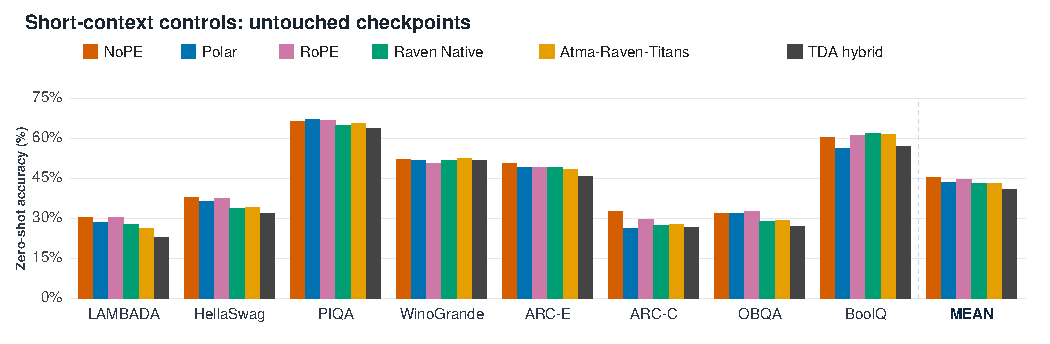
\includegraphics[width=\linewidth]{fig_downstream_candle.pdf}
\caption{Untouched zero-shot accuracy on eight 2K controls (22,939 examples per model). The rightmost group gives unweighted task means. Raven variants and TDA hybrid are separately optimized references. Table~\ref{table:gamma_downstream_full} reports the inference-cap comparison.}
\label{fig:short_context_controls}
\end{figure}

Table~\ref{tab:systems} shows the quality--systems trade-off. Raven Native reaches 46\% BABILong at 256K and keeps BPB nearly flat. Its fixed recurrent state also avoids a sequence-length-dependent KV cache. At 128K, Atma-Raven-Titans decodes at 2.27 ms/token, compared with 16.3 ms/token for Polar. Polar instead has higher synthetic retrieval and training MFU. TDA achieves 19,851 tokens/s prefill at 128K (6.46s TTFT); autoregressive decode is omitted because upstream authors provided no cached incremental decode kernel, and prefix recomputation artificially inflates decode latency. The BABILong samples are small. Simple Wilson intervals at 256K are 20.1--37.5\% for Polar (28/100) and 36.6--55.7\% for Raven Native (46/100). Because Raven also changes model family and optimizer, these rows show practical operating points rather than isolate one causal mechanism.

\begin{table}[t]
\centering
\small
\setlength{\tabcolsep}{3.2pt}
\resizebox{\linewidth}{!}{%
\begin{tabular}{llrrrr}
\toprule
\textbf{Group} & \textbf{Model} & \textbf{Base mean} & \textbf{128K prompt} & \textbf{Decode} & \textbf{Train MFU} \\
& & (\%) & (s) & (ms/token) & (\%, 2K) \\
\midrule
Matched & NoPE & 45.1 & 1.47 & 16.4 & 42.77 \\
Matched & Polar & 43.3 & 1.62 & 16.3 & 40.44 \\
Matched & RoPE & 44.6 & 1.47 & 16.5 & 42.45 \\
Raven/AdamW & Atma-Raven-Titans & 43.1 & 1.00 & 2.27 & 30.92 \\
Raven/AdamW & Raven Native & 43.0 & 1.36 & 3.27 & 21.53 \\
\midrule
AdamW/direct & TDA hybrid & 40.6 & 6.46 & \textit{Skipped} & 38.64 \\
\bottomrule
\end{tabular}}
\caption{Short-context and systems trade-offs on one L40S. TDA uses full-prefix recomputation for TTFT; autoregressive decode is omitted due to the lack of an upstream cached incremental decode kernel. Backend differences preclude an architecture-only speed comparison. Memory complexity and allocation accounting are detailed in Appendix~\ref{appendix:systems}.}
\label{tab:systems}
\end{table}

\FloatBarrier
\section{Checkpoint Variability and Retention-Horizon Audit}
\label{sec:retention_audit}

\begin{figure}[!ht]
\centering
\includegraphics[width=\linewidth]{fig_nope_pretrain_loss.pdf}
\caption{NoPE 2K validation trajectories are nearly identical, yet the checkpoints' 256K NLL values are 10.77, 9.90, and 4.07. The two L40S runs differ in microbatch size. The L4 run also differs in device class.}
\label{fig:environment}
\end{figure}

Figure~\ref{fig:environment} shows the trigger for a post-hoc audit. Three NoPE runs finish at 2.8126, 2.8128, and 2.8160 validation nats at 2K, yet reach 10.77, 9.90, and 4.07 NLL at 256K. The runs were not initialized from a recorded common seed, so the comparison establishes checkpoint variability, not a device-class treatment effect. Evaluation replays, a microbatch control, and deterministic fixtures ruled out several immediate explanations but did not identify the origin (Appendix~\ref{appendix:environment}).

\subsection{Parameter inspection}
We inspect the retention branch via the zero-input operating point $\gamma_0=\sigma(b_\gamma+b_{\rm init})$ and half-life $H_{1/2}=\log(1/2)/\log\gamma_0$ across all eight per-layer memory heads. The promoted NoPE checkpoint contains one Block 2 head with a 21.01M-token half-life, and Polar contains one at 3.07M tokens, whereas the L4 NoPE maximum is 185 tokens and Atma-Raven-Titans stays below 41.4 tokens. Because $W_\gamma$ is nonzero, runtime retention also depends on activations; this parameter scan serves as a diagnostic operating point. Outliers persist after BABILong fine-tuning (20.86M in NoPE, 3.05M in Polar).

\subsection{Single-head intervention and full re-evaluation}
To test causality, we first conducted a paired multi-clamp sweep over candidate caps on the single highest zero-input operating point: checkpoint-local percentiles (\texttt{p90}, \texttt{p99}) and absolute half-life ceilings (\texttt{hl:256}, \texttt{hl:512}) across sequence lengths from 2K to 256K (Table~\ref{table:gamma_sweep_full}). While \texttt{p99} failed on saturated models because the 99th percentile was still dominated by the outlier ($H_{1/2} \approx 484$k tokens), the 256-token half-life cap $\gamma_{\max}=2^{-1/256}=0.997296$ gave the largest long-distance cross-entropy reduction while keeping 2K clean-loss drift within the $0.05$-nat guardrail. In this same-process paired sweep, clean NLL at 256K fell from 12.003 to 1.138 for NoPE and from 1.252 to 1.057 for Polar. Needle cross-entropy fell from 12.20 to 6.05 and from 2.39 to 1.71, respectively. RoPE changed only from 6.16 to 6.02 and lost short-range retrieval, providing an empirical negative control.

We then used the selected 256-token ceiling to re-evaluate downstream tasks, retrieval, fixed-target BPB, and BABILong across the matched attention variants. Table~\ref{tab:gamma_rebench} gives the intervention endpoints; Appendix~\ref{appendix:retention_audit} provides the complete before/after curves and numerical tables. A sweep over cap ceilings $H\in\{128,256,512,1024\}$ confirms optimal rescue at $H=256$. Applying $H=256$ to alternative same-layer heads (the second-highest $H_0$ head or a random head) yields $0.0$ likelihood recovery (NoPE 256K BPB remains at $7.53$--$7.62$), proving the intervention is strictly head-specific (Appendix~\ref{appendix:pat_feedback}). All 15 jobs completed without an out-of-memory failure.

\begin{table}[!ht]
\centering
\small
\setlength{\tabcolsep}{2.6pt}
\resizebox{\linewidth}{!}{%
\begin{tabular}{lrrrrr}
\toprule
\textbf{Model} & \textbf{Max $H_{1/2}$} & \textbf{Base mean} & \textbf{256K BPB} & \textbf{256K retrieval tok./exact} & \textbf{256K BABI} \\
\midrule
NoPE & 21.01M & 45.15 $\rightarrow$ 45.10 & 8.097 $\rightarrow$ \textbf{1.595} & 0.60/0.00 $\rightarrow$ 0.93/0.00 & 0 $\rightarrow$ \textbf{39} \\
Polar & 3.07M & 43.29 $\rightarrow$ 43.25 & 1.825 $\rightarrow$ \textbf{1.501} & 34.37/9.00 $\rightarrow$ \textbf{47.07/16.33} & 28 $\rightarrow$ \textbf{42} \\
RoPE & 682 & 44.60 $\rightarrow$ 44.66 & 2.512 $\rightarrow$ 2.460 & 0.00/0.00 $\rightarrow$ 0.00/0.00 & 14 $\rightarrow$ 11 \\
\bottomrule
\end{tabular}}
\caption{Inference-only retention diagnostic. Results show archived baseline $\rightarrow$ one-head 256-token half-life cap. Base mean averages eight 2K tasks (\%). Retrieval is token/exact accuracy (\%), BABI is macro exact match, and BPB averages three fixed-target datasets. The cap is a probe, not a proposed trained model.}
\label{tab:gamma_rebench}
\end{table}

The intervention largely removes NoPE's likelihood collapse and raises BABILong to 54/45/37/35/39\% at 16/32/64/128/256K (from 21/6/0/0/0\%). However, NoPE's exact natural-text retrieval remains zero beyond 8K and zero overall at 256K, demonstrating that state stability alone is insufficient for associative recall. For Polar, the cap improves 256K token retrieval by 12.70 points, overall exact retrieval by 7.33 points, and BABILong by 14 points, while mean BPB degradation drops from $1.26\times$ to $1.03\times$ with $<0.06$ points change on 2K controls. RoPE shows no retrieval recovery and its BABILong score falls. The cap thus identifies excessive retention as a primary mediator of likelihood collapse without serving as a generic benchmark boost.

\subsection{Retention intervention in the fresh pairs}
The fresh runs in Table~\ref{tab:replication_main} also received the same checkpoint-local cap. NoPE's maximum zero-input half-lives were 135k and 5.78M tokens; the cap reduced 256K BPB from 3.898/5.256 to 1.506/1.490, but reduced token retrieval from 4.83/12.13\% to 0.73/7.07\%. Polar's maxima were 272 and 231 tokens, and its metrics changed little. Thus the NoPE likelihood repair repeats across independent runs, while Polar's primary cap gain does not repeat, and neither architecture shows a general retrieval benefit from the cap (Appendix~\ref{appendix:seed_replication}).

\subsection{What this audit resolves and delimits}
These investigations resolve key mechanistic questions: Polar's advantage over temperature scaling alone is established (+22.18\%) and the retention cap benefit is strictly head-specific (Appendix~\ref{appendix:pat_feedback}). What remains open is the exact pretraining optimization dynamics that first spawn the outlier, and whether bounded train-time parameterization stabilizes early training without degrading long timescales. Resolving them requires varying architecture, optimizer, and sequence length from step zero.

\section{Limitations and Conclusion}
The evidence covers one model scale and 2K pretraining, two fresh NoPE/Polar pairs, and no seed-matched RoPE replication. Shared retrieval haystacks, 18 fixed BPB targets, and single-sequence serving limit coverage. Teacher-forced retrieval and adapted BABILong answer different questions; every model loses exact FinePDFs retrieval at extreme lengths. Raven and TDA use separate AdamW recipes; TDA decode is omitted due to un-cached upstream serving.

Within this scope, memory improves Polar retrieval in every factorial contrast, and Polar exceeds NoPE across seeds and on 30 independent documents. A single-head cap repairs NoPE likelihood collapse across runs without acting as an unconditional benchmark boost. Prospective component controls confirm Polar's advantage over learned length temperatures alone (+22.18\%), establishing the value of its directional decomposition for long-context language modeling.

\subsection*{AI Use Statement}
Generative AI assisted diagnostic scripts, manuscript structure, and log aggregation. The authors ran benchmarks on the listed hardware; AI did not generate datasets or train models. The authors verified all mathematics, code, and values against original derivations and source logs, taking full responsibility for all claims under the ICLR 2027 policy.

\subsection*{Reproducibility Statement}
Sections 3--4 specify models and training. Appendices~\ref{appendix:protocol}, \ref{appendix:seed_replication}, \ref{appendix:retention_audit}, and~\ref{appendix:pat_feedback} give evaluation protocols, replications, interventions, and follow-up controls; the remaining appendices provide detailed results and implementations. The public artifact at \url{https://github.com/kreasof-ai/atma} contains configurations, logs, checkpoint manifests, benchmark payloads, clamp specifications, and machine-checked proof skeletons.

\clearpage
\bibliography{colm2026_conference,iclr2027_additions}
\bibliographystyle{iclr2027_conference}

\appendix
\section{Theoretical Framing}
\label{appendix:theory}

These are sufficient-condition results. They establish noise-odds and norm bounds under explicit assumptions. They do not establish distributional invariance or replace the empirical evidence.

\subsection{Extreme-value null floor}

\begin{assumption}[Sub-Gaussian noise scores]
For irrelevant keys $j\in\mathcal N_n$, $|\mathcal N_n|\leq n$, scores $X_j$ are mean-zero and $v^2$-sub-Gaussian: $\mathbb E\exp(tX_j)\leq\exp(v^2t^2/2)$ for all $t\in\mathbb R$.
\end{assumption}

Let the Polar null floor be $\nu_n=b+s\sqrt{\log(n+1)}$ with $b,s\geq0$.

\begin{proposition}[Noise exceedances]
Under Assumption 1,
\begin{equation}
\mathbb E\!\left[\sum_{j\in\mathcal N_n}{\bf1}\{X_j>\nu_n\}\right]
\leq n\exp\!\left(-\frac{\nu_n^2}{2v^2}\right).
\end{equation}
If $s\geq\sqrt2v$ this is $O(1)$; if the inequality is strict it decays polynomially.
\end{proposition}

\begin{proof}
Apply the sub-Gaussian tail bound to each key and sum. Since $b\geq0$, $\nu_n^2\geq s^2\log(n+1)$.
\end{proof}

Unlike TDA, Polar retains sub-threshold keys. With temperature $\theta_n=1+a\log n$, define the unnormalized noise-to-null odds $R_n=\sum_{j\in\mathcal N_n}\exp(\theta_n(X_j-\nu_n))$.

\begin{proposition}[Vanishing null odds]
Suppose $s>c>\sqrt2v$ and the null floor is $s\sqrt{\log(n+1)}$ up to a nonnegative offset. With probability tending to one,
\begin{equation}
R_n\leq n\exp\!\left(-(1+a\log n)(s-c)\sqrt{\log n}\right).
\end{equation}
For $a>0$, the bound converges to zero faster than any inverse polynomial.
\end{proposition}

\begin{proof}
A union bound gives $\Pr[\max_jX_j>c\sqrt{\log(n+1)}]\leq n(n+1)^{-c^2/(2v^2)}\to0$. On the complementary event, every noise score is at least $(s-c)\sqrt{\log n}$ below the floor. Bound each summand and sum over at most $n$ keys.
\end{proof}

\subsection{Bounded channels and recurrent state}

\begin{proposition}[Bounded Polar readout]
For $c_i=s_i/\max(\lVert s_i\rVert_2,\varepsilon)$, $\lVert c_i\rVert_2\leq1$. For $\mu_i=\tanh(\beta\log(1+m_{{\rm eff},i}))$, $\mu_i\in[0,1)$ when $\beta,m_{{\rm eff},i}\geq0$. A distribution uniform over $m$ real keys has participation ratio $m$.
\end{proposition}

\begin{proof}
The first two claims follow from the denominator and range of $\tanh$. Uniform weights satisfy $(\sum_{j=1}^m(1/m)^2)^{-1}=m$.
\end{proof}

\begin{assumption}[Contractive memory]
For every $t$, $\lVert q_t\rVert_2=\lVert k_t\rVert_2=1$, $\lVert v_t\rVert_2\leq V$, $0\leq\beta_t\leq1$, and $0\leq\gamma_t\leq\bar\gamma<1$.
\end{assumption}

\begin{proposition}[Length-bounded state]
For recurrence~\eqref{eq:memory},
\begin{equation}
\lVert M_t\rVert_F\leq\bar\gamma^t\lVert M_0\rVert_F+\frac{V}{1-\bar\gamma}.
\end{equation}
\end{proposition}

\begin{proof}
$I-\beta_tk_tk_t^\top$ has spectral norm at most one and $\lVert\beta_tv_tk_t^\top\rVert_F\leq V$. Thus $\lVert M_t\rVert_F\leq\bar\gamma\lVert M_{t-1}\rVert_F+V$; unrolling gives the result.
\end{proof}

The Lean artifact checks the finite-sum, exponential-monotonicity, bounded-channel composition, and invariant-set induction steps. It takes the sub-Gaussian tail, high-probability margin, and one-step contraction as premises. It is therefore a machine-checked proof skeleton, not end-to-end formal verification. The learned Polar conditions $b\geq0$ and $s>c>\sqrt2v$ require an empirical head-wise audit before they can be asserted for a trained checkpoint. Likewise, $\gamma_t=\sigma(W_\gamma x_t+b_\gamma)$ establishes only $0<\gamma_t<1$ at any finite logit; it does not supply one sequence-uniform $\bar\gamma<1$. Appendix~\ref{appendix:retention_audit} shows that the distinction is practically material: individual zero-input operating points can imply million-token half-lives, although that parameter-only scan does not by itself bound activation-conditioned runtime gates.

\section{Regularization Modes}
\label{appendix:reg_modes}

The factorial grid varies a representation regularizer applied to the model's signature stream. For every non-baseline mode, the sweep uses the same weight $\alpha_{\rm sig}=0.01$ and optimizes
\begin{equation}
\mathcal L=(1-\alpha_{\rm sig})\mathcal L_{\rm LM}
+\alpha_{\rm sig}\mathcal L_{\rm reg}
+\lambda_{\rm dist}\mathcal L_{\rm dist}.
\end{equation}
The weak and strong modes follow the two SIGReg families introduced by Weak-SIGReg~\citep{weak_sigreg2026} and LeJEPA's strong SIGReg objective~\citep{lejepa2025}. The discrete and zipfian modes are local variants that combine those ideas with stronger geometric priors. Table~\ref{table:reg_modes} defines all five sweep settings.

\begin{table}[!ht]
\centering
\small
\begin{tabular}{p{0.17\linewidth}p{0.76\linewidth}}
\toprule
\textbf{Mode} & \textbf{Meaning in the sweep} \\
\midrule
\texttt{baseline} & No signature-stream regularization; equivalently, $\alpha_{\rm sig}=0$. \\
\texttt{weak} & Weak SIGReg: center a random sketch of the token representations and match its covariance to the identity, $\lVert\operatorname{Cov}(Sx)-I\rVert_F$. This encourages decorrelated, unit-variance features at low cost. \\
\texttt{strong} & Strong SIGReg: project representations onto random one-dimensional directions and match their empirical characteristic functions to the standard Gaussian characteristic function over a fixed frequency grid. \\
\texttt{discrete} & Local variant: normalize each representation to the sphere of radius $\sqrt d$, then apply weak covariance matching. This preserves whitening pressure while encouraging fixed-norm, discrete-code-like directions. \\
\texttt{zipfian} & Local variant: normalize directions for an orthogonality penalty, then match sorted representation magnitudes to a Zipf profile $r^{-1}$. This biases the signature stream toward heavy-tailed feature use rather than uniform energy allocation. \\
\bottomrule
\end{tabular}
\caption{Regularization modes in the 120-cell factorial sweep. Weak and strong are SIGReg-style covariance and distribution-matching objectives; discrete and zipfian are exploratory local variants.}
\label{table:reg_modes}
\end{table}
\FloatBarrier

\section{Polar Attention Implementation}
\label{appendix:polar_implementation}

\subsection{Design provenance and scope}
Before integration, the Polar choices were developed by falsifying simpler alternatives in a standalone synthetic sandbox. Additive soft counts accumulated small per-key leakage with sequence length; thresholds based on a fixed number of standard deviations retained a constant fraction of noise keys; a fixed null logit was eventually overtaken by the maximum noise score; and an unbounded $\log m$ magnitude exposed the output projection to values beyond its training range. These failures motivated participation ratio, the $\sqrt{\log n}$ null floor, and the bounded $\tanh(\beta\log(1+m))$ map. The standalone prototype was subsequently removed and is not part of the released artifact. We therefore use these tests as design provenance, not as model-scale component ablations or independently reproducible benchmark evidence. The integrated equations, materialized oracle, streaming implementation, and parity tests described below are retained.

\subsection{Integrated component pilot}
\label{appendix:polar_components}
We subsequently ran a matched network-level component study using the promoted Polar+memory recipe. Each 378.22M-parameter model received 1B tokens at length 2K with the same initialization and data seed; evaluation used the same documents, retrieval prompts, and seed. ``Fixed null slope'' sets only the nonnegative $\sqrt{\log(n+1)}$ coefficient in Equation~\ref{eq:length} near zero; the null base and null vector remain learned. Table~\ref{table:polar_components} reports the prespecified metrics. The clean and junk columns are NLL in nats/token on coherent FinePDFs and the concatenated FineWeb-Edu validation stream, respectively.

\begin{table}[!ht]
\centering
\small
\setlength{\tabcolsep}{3.5pt}
\resizebox{\linewidth}{!}{%
\begin{tabular}{lrrrrrr}
\toprule
\textbf{Polar variant} & \textbf{Val. NLL} & \textbf{Clean 2K} & \textbf{Clean 64K} & \textbf{Junk 2K} & \textbf{Junk 64K} & \textbf{Needle 2K / 64K (\%)} \\
\midrule
Full Polar & 3.1688 & 2.810 & 2.047 & 3.110 & 3.129 & 91.25 / 77.50 \\
Direction only & \textbf{3.1629} & 2.709 & 1.982 & \textbf{3.103} & \textbf{3.124} & 91.25 / 71.25 \\
Constant magnitude & 3.1717 & 2.734 & \textbf{1.924} & 3.113 & 3.134 & 92.50 / 16.25 \\
Fixed null slope & 3.1741 & 2.725 & 1.938 & 3.117 & 3.142 & \textbf{96.25 / 91.25} \\
Fixed temperature gain & 3.1695 & \textbf{2.707} & 1.967 & 3.111 & 3.155 & 93.75 / 16.25 \\
\bottomrule
\end{tabular}}
\caption{Single-seed, 1B-token Polar component attribution. Needle values are teacher-forced five-token accuracy over 16 trials per length. All variants share the same seed, but this design does not estimate variation across training seeds.}
\label{table:polar_components}
\end{table}

Ordinary language-model losses are tightly grouped: validation NLL spans only 0.0112 nats, and every intervention improves clean NLL relative to Full Polar at matched lengths. Retrieval is more diagnostic. Direction only retains most of the 64K accuracy (71.25\% versus 77.50\%), whereas constant magnitude and fixed temperature gain each fall to 16.25\%. Thus the direction-only path carries most of the retrieval signal, and the learned length temperature is important. An uninformative constant count signal is harmful, but this study does not establish that the count channel is always necessary.

Unexpectedly, fixing the length-dependent null slope near zero gives the best retrieval at every evaluated length and reaches 91.25\% at 64K, while slightly worsening validation and junk-stream NLL. One plausible explanation is that a slope learned only through 2K over-rejects distant relevant keys when extrapolated, especially because this recipe disables the explicit distractor-alignment objective. The matched seed makes an independently luckier initialization an unlikely explanation for this contrast, but one training seed and 16 retrieval trials per length cannot establish a population-level effect. We therefore retain the prespecified Full Polar model for the confirmatory comparison and treat null calibration as unresolved. Future work should replicate the contrast across seeds and larger retrieval samples, measure null mass by head versus length, and test bounded or score-adaptive null formulations. The synthetic provenance above and this integrated pilot answer different questions: the former motivates the asymptotic design, while the latter shows that its learned finite-training calibration is not yet empirically optimal.

\subsection{Numerical oracle}
The materialized PyTorch path forms the masked real-key logits and virtual null logit in FP32, applies a single softmax, and computes the direction and magnitude channels from the resulting weights. It is used as a numerical oracle for forward and backward tests, not as the production long-context path, because materializing the $T\times T$ score matrix is memory-prohibitive at the evaluated lengths.

\subsection{Streaming sufficient statistics}
The Triton kernel follows the online-max strategy used by FlashAttention-style kernels. For one query row, it streams $K,V$ blocks and retains only four FP32 statistics: the running maximum $M$, real-key exponential sum $L$, squared exponential sum $Q_2$, and unnormalized value sum $S$. If a new block changes the row maximum, $\alpha=\exp(M_{\rm old}-M_{\rm new})$ rescales each statistic as shown in Table~\ref{table:polar_streaming_state}.

\begin{table}[!ht]
\centering
\small
\begin{tabular}{lll}
\toprule
\textbf{State} & \textbf{Online update} & \textbf{Use after streaming} \\
\midrule
$M$ & $M\leftarrow\max(M,\max a)$ & Stable common logit origin \\
$L$ & $L\leftarrow\alpha L+\sum_jp_j$ & Real-key softmax mass \\
$Q_2$ & $Q_2\leftarrow\alpha^2Q_2+\sum_jp_j^2$ & $n_{\rm eff}=L^2/Q_2$ \\
$S$ & $S\leftarrow\alpha S+\sum_jp_jv_j$ & Direction numerator \\
\bottomrule
\end{tabular}
\caption{Streaming state for one Polar query row, where $a$ is the current logit block and $p_j=\exp(a_j-M_{\rm new})$. The squared accumulator must rescale by $\alpha^2$.}
\label{table:polar_streaming_state}
\end{table}

After the real keys are consumed, the virtual null is folded in as one additional softmax entry. Let $p_0=\exp(t_i\nu_i-M)$ and $Z=L+p_0$. The kernel obtains
\begin{equation}
c_i=\operatorname{normalize}(S+p_0v_{\rm null}),\qquad
n_{{\rm eff},i}=\frac{L^2}{Q_2},\qquad
m_{{\rm eff},i}=n_{{\rm eff},i}\frac{L}{Z}.
\end{equation}
The common factor $1/Z$ cancels under radial normalization of the direction numerator. The production kernel evaluates the magnitude with $2\sigma(2x)-1=\tanh x$ and saves $(M,L,Q_2,S)$ for the backward pass. Listing~\ref{lst:polar_triton} gives the algorithmic core; pointer arithmetic, launch metadata, and backward code are omitted.

\begin{lstlisting}[language=Python,caption={Schematic core of the block-streamed Triton forward pass.},label={lst:polar_triton}]
@triton.jit
def polar_fwd_core(q, K, V, n_i, temp, nullv, beta,
                   BLOCK_N: tl.constexpr, DK: tl.constexpr):
    M  = tl.full([BLOCK_M], -1e38, tl.float32)
    L  = tl.zeros([BLOCK_M], tl.float32)
    Q2 = tl.zeros([BLOCK_M], tl.float32)
    S  = tl.zeros([BLOCK_M, DK], tl.float32)

    for start in range(0, n_i, BLOCK_N):
        k, v, valid = load_kv_block(K, V, start, n_i)
        a = tl.where(valid, temp[:, None] * dot(q, k), -1e38)
        M_new = tl.maximum(M, tl.max(a, axis=1))
        alpha = tl.exp(M - M_new)
        p = tl.where(valid, tl.exp(a - M_new[:, None]), 0.0)
        L  = alpha * L + tl.sum(p, axis=1)
        Q2 = alpha * alpha * Q2 + tl.sum(p * p, axis=1)
        S  = alpha[:, None] * S + tl.dot(p, v)
        M = M_new

    # Fold in the learned virtual null as one extra entry.
    M_new = tl.maximum(M, temp * nullv)
    alpha = tl.exp(M - M_new)
    L, Q2, S = alpha * L, alpha * alpha * Q2, alpha[:, None] * S
    p_null = tl.exp(temp * nullv - M_new)
    Z = L + p_null

    direction = normalize(S + p_null[:, None] * v_null)
    n_eff = L * L / tl.maximum(Q2, eps)
    m_eff = n_eff * L / tl.maximum(Z, eps)
    magnitude = 2 * tl.sigmoid(2 * beta * tl.log(1 + m_eff)) - 1
    save_for_backward(M_new, L, Q2, S)
\end{lstlisting}

This removes the quadratic \emph{score-matrix storage}. Full-context prefill still performs quadratic query-key arithmetic. The kernel is cross-checked against the materialized PyTorch oracle in FP32 accumulation before lower-precision outputs are accepted.

\section{Evaluation Protocols}
\label{appendix:protocol}

Stage I contains 120 approximately 370--378M-parameter runs trained for 1,900 steps of 524,288 tokens at sequence length 2,048 on FineWeb-Edu. Stage II contains three matched attention models trained for 18,722 such steps (9.816B tokens). The five original promoted checkpoints, the additional TDA hybrid, and ten open-weight controls are evaluated with checkpoint-exact forward paths. Stage I cells vary factorial settings and are not independent seed replicates.

\paragraph{External hybrid recipe.}
The additional TDA hybrid~\citep{huang2026threshold} has 388,641,924 parameters, width 1024, and 16 blocks: twelve local convolution blocks and four global TDA layers. Each global layer uses 16 heads of dimension 64, the upstream differential-threshold Triton reduction with normalization, and a per-head output RMS normalization. The gated-delta memory side channel shares the excitatory query/key view and values; this is one explicit integration choice, not a unique native TDA architecture. The configured threshold coefficient is 1, the ReLU power is 2, and the learned differential coefficient initializes at 0.5. The pinned TDA source revision begins \texttt{cd8ddc9d5b43}; the complete dependency revisions and checkpoint hashes are archived with the run.

Training completed 18,722 steps of 524,288 FineWeb-Edu tokens (9.816B), with the same tokenizer, sequence length 2048, and L40S device class as the promoted runs. Initialization and data seeds are 202701; microbatch size is four. AdamW uses peak learning rate $3\times10^{-4}$, minimum learning-rate fraction 0.1, warmup fraction 0.05, $(\beta_1,\beta_2)=(0.9,0.95)$, and weight decay 0.1. Final validation loss is 3.06317 nats/token. Parameter count, head geometry, integration, and optimizer differ from the matched NoPE/RoPE/Polar group, so the comparison does not isolate the attention operator.

\subsection{Raven optimizer control}
The Raven rows use AdamW optimizer because the attempted matched-schedule control did not produce a usable baseline. In the 1B-token Raven Native pilot with the Atma Muon schedule, validation loss decreased from 10.83 to 3.76 nats by step 625, then rose to 6.88 at step 1,125 and ended at 4.62; teacher-forced retrieval was 0\% at every tested length from 2K through 64K. The reported Raven Native and Atma-Raven-Titans checkpoints therefore use AdamW and remain a separate model-family/optimizer group. This is evidence about the tested Muon schedule, not a general claim that Raven cannot converge under any Muon tuning.

Retrieval crosses passkey and NIAH tasks, synthetic and FinePDFs haystacks, eight lengths from 2K through 256K, three depths, and 50 paired trials per cell. The scorer appends the complete five-token target and evaluates each position conditioned on the preceding ground-truth target tokens. Token accuracy is the fraction of correct per-position argmax predictions; exact accuracy requires all five positions to be correct. Both are teacher-forced diagnostics, not autoregressive generation. An older free-generation protocol was retired because all base checkpoints scored uniformly zero. BABILong uses answer-only fine-tuning on tasks qa1--qa10 at 0K/1K/2K and greedy exact match on ten held-out rows per task and length. Base-task controls use LAMBADA, HellaSwag, PIQA, WinoGrande, ARC-Easy, ARC-Challenge, OpenBookQA, and BoolQ. Fixed-target BPB uses FinePDFs, PG-19, and Proof-Pile. All reported processes completed without failed, OOM, unsupported, missing, or null cells.

\paragraph{Text coverage and aggregation.}
The 28,800 retrieval evaluations count six models, including TDA hybrid, each on $2\times2\times8\times3\times50=4{,}800$ trials. A single stream of concatenated FinePDFs records supplies every real-text haystack; shorter lengths use prefixes of that stream. The same 50 sample indices per task determine cues and five random digits across lengths, depths, suites, and models. These are paired placements and targets rather than independently sampled documents. Synthetic haystacks repeat the same filler. At each length, overall retrieval gives equal weight to the 12 task--suite--depth cells. Smoke runs are excluded from all reported full-evaluation means.

For primary fixed-target BPB, the evaluator selects the first qualifying documents with at least $262{,}144+256$ GPT-2 tokens: eight FinePDFs, five PG-19, and five Proof-Pile documents. Every context length predicts the same 256-token span immediately after position 262,144, giving 4,608 scored target tokens per model and length. Dataset BPB divides summed target negative log-likelihood in bits by summed UTF-8 target bytes; the reported mean weights the three datasets equally. Additional context changes the conditioning prefix rather than the target. These 18 spans provide a controlled extrapolation diagnostic, not a representative estimate over all documents in the three corpora.

For proportions we report simple Wilson intervals where they aid interpretation. These intervals treat trials as binomial observations and do not exploit the paired design or account for correlations induced by shared templates. The archived retrieval payloads retain aggregate cell counts but the BABILong payloads do not retain per-model correctness vectors, so paired bootstrap or McNemar tests cannot be reconstructed without rerunning or recovering the original predictions.

The TDA hybrid uses the same pinned benchmark revisions and budgets and a separately adapted, validation-selected BABILong checkpoint. Its checkpoint-exact direct scorer verifies dependency revisions and checkpoint keys. All nine pipeline stages completed, including retrieval through 256K without OOM.

\begin{landscape}
\section{Complete Factorial Sweep}
\label{appendix:full_ablation}

Table~\ref{table:ablation_appendix} retains all 120 factorial cells; the main paper reports only the recipe transitions needed to justify promotion.
\begingroup
\normalsize
\setlength{\tabcolsep}{5pt}
\input{appendix_table.tex}
\endgroup
\end{landscape}

\section{Seed-Paired Replication}
\label{appendix:seed_replication}

We trained four fresh 378M-parameter checkpoints: paired NoPE and Polar runs at seeds 202701 and 202702. Every run used 18,722 steps of 524,288 tokens (9.816B tokens), sequence length 2,048, the L40S configuration with microbatch size four, and the same data order within each seed pair. Final validation NLL differed by architecture but was stable across seeds (Table~\ref{table:replication_endpoints}). Checkpoints and evaluation datasets were pinned to immutable Hub revisions.

The follow-up was intentionally restricted to the two diagnostics relevant to the retention hypothesis: teacher-forced retrieval and fixed-target BPB. We did not run downstream tasks or BABILong. For each checkpoint we compared the untouched model with the checkpoint-local 256-token cap on its largest parameter-only zero-input retention head. Retrieval used the same synthetic/FinePDFs, passkey/NIAH, length, depth, sample, target, and seed grid as the primary evaluation: 38,400 trials across the eight model--condition combinations. Fixed-target BPB used eight qualifying FinePDFs documents and five qualifying documents each from PG-19 and Proof-Pile; document hashes were identical across models and conditions. All 24 jobs completed without an OOM or failed cell.

\begin{table}[ht]
\centering
\small
\setlength{\tabcolsep}{3.2pt}
\resizebox{\linewidth}{!}{%
\begin{tabular}{llrrrr}
\toprule
\textbf{Seed} & \textbf{Architecture} & \textbf{Final val. NLL} & \textbf{Max $H_{1/2}$} & \textbf{256K BPB} & \textbf{256K retrieval tok./exact} \\
\midrule
202701 & NoPE  & 2.81164 & 135k (B2/H2)  & 3.898 $\rightarrow$ 1.506 & 4.83/0.00 $\rightarrow$ 0.73/0.00 \\
202701 & Polar & 2.85661 & 272 (B10/H7) & 1.644 $\rightarrow$ 1.644 & 16.97/0.00 $\rightarrow$ 16.53/0.00 \\
202702 & NoPE  & 2.81474 & 5.78M (B2/H3) & 5.256 $\rightarrow$ 1.490 & 12.13/0.00 $\rightarrow$ 7.07/0.00 \\
202702 & Polar & 2.85417 & 231 (B6/H4)  & 1.760 $\rightarrow$ 1.762 & 20.90/3.83 $\rightarrow$ 21.13/3.83 \\
\bottomrule
\end{tabular}}
\caption{Seed-level replication endpoints. Each metric reports untouched $\rightarrow$ capped evaluation. Retrieval averages passkey and NIAH, three depths, and synthetic and real-text suites; values are percentages. $H_{1/2}$ is the maximum parameter-only zero-input operating point, with zero-indexed block/head coordinates.}
\label{table:replication_endpoints}
\end{table}

\begin{table}[ht]
\centering
\scriptsize
\setlength{\tabcolsep}{2.7pt}
\resizebox{\linewidth}{!}{%
\begin{tabular}{lllrrrrrrrr}
\toprule
\textbf{Architecture} & \textbf{Condition} & \textbf{Metric} & \textbf{2K} & \textbf{4K} & \textbf{8K} & \textbf{16K} & \textbf{32K} & \textbf{64K} & \textbf{128K} & \textbf{256K} \\
\midrule
NoPE & untouched & Retrieval token & 99.00 & 72.50 & 51.62 & 47.62 & 42.42 & 33.85 & 19.42 & 8.48 \\
NoPE & capped    & Retrieval token & 98.55 & 85.27 & 82.52 & 56.53 & 34.05 & 17.77 & 8.50 & 3.90 \\
Polar & untouched & Retrieval token & 98.65 & 95.77 & 97.52 & 89.17 & 67.32 & 51.30 & 27.88 & 18.93 \\
Polar & capped    & Retrieval token & 98.70 & 95.78 & 97.77 & 89.48 & 67.40 & 52.25 & 28.22 & 18.83 \\
\midrule
NoPE & untouched & Retrieval exact & 95.00 & 61.33 & 43.25 & 39.25 & 24.50 & 9.08 & 0.75 & 0.00 \\
NoPE & capped    & Retrieval exact & 92.92 & 62.58 & 55.25 & 19.92 & 5.08 & 0.08 & 0.00 & 0.00 \\
Polar & untouched & Retrieval exact & 93.58 & 84.25 & 88.67 & 70.08 & 18.33 & 12.42 & 4.83 & 1.92 \\
Polar & capped    & Retrieval exact & 93.83 & 84.42 & 89.50 & 70.17 & 19.08 & 14.33 & 5.17 & 1.92 \\
\midrule
NoPE & untouched & Mean BPB & 1.379 & 1.442 & 2.016 & 2.590 & 3.346 & 3.619 & 3.902 & 4.577 \\
NoPE & capped    & Mean BPB & 1.397 & 1.397 & 1.416 & 1.420 & 1.445 & 1.435 & 1.459 & 1.498 \\
Polar & untouched & Mean BPB & 1.432 & 1.424 & 1.448 & 1.458 & 1.522 & 1.557 & 1.617 & 1.702 \\
Polar & capped    & Mean BPB & 1.435 & 1.426 & 1.449 & 1.459 & 1.523 & 1.558 & 1.618 & 1.703 \\
\bottomrule
\end{tabular}}
\caption{Complete replication curves, descriptively averaged over the two seeds. Retrieval metrics are percentages and give equal weight to the 12 task--suite--depth cells at each length. BPB gives equal weight to FinePDFs, PG-19, and Proof-Pile. These two seeds do not support a population uncertainty estimate.}
\label{table:replication_curves}
\end{table}

Both NoPE checkpoints developed much longer zero-input horizons than either Polar checkpoint. Their mean BPB growth from 2K to 256K was $3.32\times$ when untouched and $1.07\times$ when capped; the cap repaired the likelihood collapse in both seeds. It did not rescue retrieval: seed-averaged NoPE token accuracy fell from 33.85\% to 17.77\% at 64K and from 8.48\% to 3.90\% at 256K. Conversely, Polar had $1.19\times$ BPB growth in both conditions and nearly overlapping retrieval curves because its maxima were already near the selected ceiling. At 256K, every condition had zero exact real-text retrieval; Polar's 1.92\% overall exact mean came from the synthetic suite in seed 202702. The replication therefore supports excessive retention as a checkpoint-specific likelihood-collapse mechanism, especially for NoPE, while refuting a general expectation that the cap improves retrieval or that every Polar checkpoint develops a comparable outlier.

\section{Retrieval Breakdown}
\label{appendix:retrieval}

\begin{figure}[h]
\centering
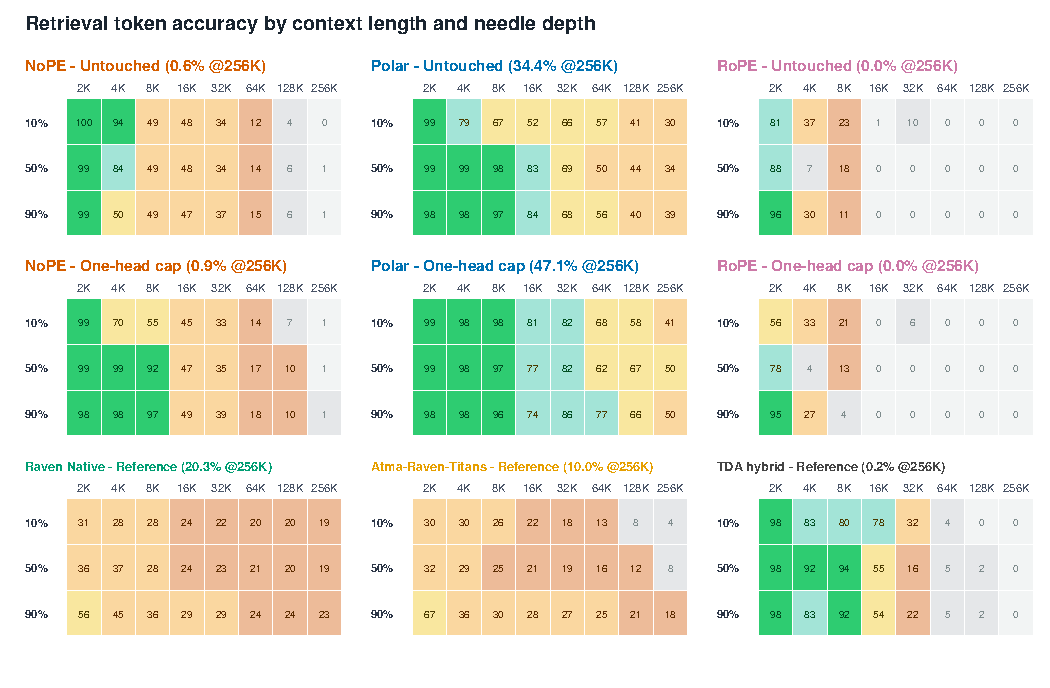
\includegraphics[width=\linewidth]{fig_niah_heatmap.pdf}
\caption{Retrieval depth sweeps for the three matched attention variants before and after the one-head retention cap, followed by untouched Raven Native, Atma-Raven-Titans, and TDA hybrid reference panels. Each cell is teacher-forced token accuracy averaged over passkey and NIAH and over synthetic and FinePDFs haystacks. The reference row contains separate AdamW recipes without clamping.}
\label{fig:retrieval_depth_sweeps}
\end{figure}

\begin{table}[t]
\centering
\small
\setlength{\tabcolsep}{4pt}
\resizebox{\linewidth}{!}{%
\begin{tabular}{llrrrrrrrr}
\toprule
\textbf{Model} & \textbf{Haystack} & \textbf{2K} & \textbf{4K} & \textbf{8K} & \textbf{16K} & \textbf{32K} & \textbf{64K} & \textbf{128K} & \textbf{256K} \\
\midrule
Polar & Synthetic & 99.1 & 98.4 & 97.1 & 97.0 & 94.9 & 92.3 & 80.3 & 68.4 \\
 & FinePDFs & 98.6 & 86.3 & 77.9 & 49.1 & 40.7 & 16.3 & 3.2 & 0.3 \\
NoPE & Synthetic & 99.1 & 98.7 & 97.7 & 94.9 & 70.3 & 26.5 & 10.2 & 1.2 \\
 & FinePDFs & 99.3 & 52.9 & 0.0 & 0.0 & 0.0 & 0.0 & 0.0 & 0.0 \\
RoPE & Synthetic & 81.7 & 44.9 & 34.5 & 0.8 & 6.8 & 0.1 & 0.0 & 0.0 \\
 & FinePDFs & 94.8 & 4.7 & 0.2 & 0.0 & 0.0 & 0.0 & 0.0 & 0.0 \\
Atma-Raven-Titans & Synthetic & 63.0 & 60.7 & 53.8 & 46.9 & 41.7 & 35.8 & 25.9 & 19.3 \\
 & FinePDFs & 23.2 & 2.6 & 0.7 & 0.2 & 1.4 & 0.5 & 1.6 & 0.7 \\
Raven Native & Synthetic & 60.1 & 57.7 & 52.7 & 48.3 & 44.3 & 40.9 & 38.9 & 35.1 \\
 & FinePDFs & 22.1 & 15.4 & 8.2 & 3.3 & 5.3 & 2.9 & 3.7 & 5.4 \\
TDA hybrid & Synthetic & 96.6 & 96.4 & 94.6 & 83.7 & 25.9 & 6.3 & 2.5 & 0.5 \\
 & FinePDFs & 99.0 & 74.9 & 82.5 & 41.2 & 20.5 & 3.1 & 0.3 & 0.0 \\
\bottomrule
\end{tabular}}
\caption{Untouched teacher-forced target-token retrieval accuracy (\%). Each entry averages two tasks and three depths, with 50 trials per cell. Only full evaluations enter these means; smoke runs are excluded.}
\label{table:retrieval_breakdown}
\end{table}

\begin{table}[t]
\centering
\small
\setlength{\tabcolsep}{4pt}
\resizebox{\linewidth}{!}{%
\begin{tabular}{llrrrrrrrr}
\toprule
\textbf{Model} & \textbf{Haystack} & \textbf{2K} & \textbf{4K} & \textbf{8K} & \textbf{16K} & \textbf{32K} & \textbf{64K} & \textbf{128K} & \textbf{256K} \\
\midrule
Polar & Synthetic & 96.3 & 92.3 & 86.3 & 86.0 & 76.0 & 65.7 & 26.3 & 18.0 \\
 & FinePDFs & 93.0 & 67.3 & 62.7 & 12.0 & 0.0 & 0.0 & 0.0 & 0.0 \\
NoPE & Synthetic & 95.3 & 93.7 & 88.7 & 78.0 & 23.7 & 4.7 & 0.7 & 0.0 \\
 & FinePDFs & 96.7 & 18.0 & 0.0 & 0.0 & 0.0 & 0.0 & 0.0 & 0.0 \\
RoPE & Synthetic & 42.3 & 4.3 & 0.7 & 0.0 & 0.0 & 0.0 & 0.0 & 0.0 \\
 & FinePDFs & 77.3 & 0.0 & 0.0 & 0.0 & 0.0 & 0.0 & 0.0 & 0.0 \\
Atma-Raven-Titans & Synthetic & 8.0 & 5.7 & 3.3 & 2.0 & 0.7 & 0.3 & 0.0 & 0.0 \\
 & FinePDFs & 4.7 & 0.0 & 0.0 & 0.0 & 0.0 & 0.0 & 0.0 & 0.0 \\
Raven Native & Synthetic & 2.0 & 1.0 & 0.3 & 0.0 & 0.0 & 0.0 & 0.0 & 0.0 \\
 & FinePDFs & 0.0 & 0.0 & 0.0 & 0.0 & 0.0 & 0.0 & 0.0 & 0.0 \\
TDA hybrid & Synthetic & 86.0 & 84.3 & 76.0 & 41.3 & 0.3 & 0.0 & 0.0 & 0.0 \\
 & FinePDFs & 95.0 & 25.3 & 45.7 & 2.0 & 1.0 & 0.0 & 0.0 & 0.0 \\
\bottomrule
\end{tabular}}
\caption{Untouched teacher-forced exact five-token retrieval accuracy (\%). Each entry averages two tasks and three depths, with 50 trials per cell. Only full evaluations enter these means; smoke runs are excluded.}
\label{table:retrieval_exact_breakdown}
\end{table}

Figure~\ref{fig:retrieval_depth_sweeps} shows variation by needle depth across all six models, including TDA hybrid. Tables~\ref{table:retrieval_breakdown} and~\ref{table:retrieval_exact_breakdown} separate partial target-token signal from exact five-token recall. Every tested model eventually reaches 0.0\% exact retrieval on real-text haystacks under unadapted length extrapolation:
\begin{itemize}
\item \textbf{Raven Native and Atma-Raven-Titans:} Raven Native scores 0.0\% on FinePDFs at every tested length and no more than 2.0\% on synthetic haystacks. Atma-Raven-Titans scores 4.7\% at 2K on FinePDFs and 0.0\% from 4K onward.
\item \textbf{TDA hybrid:} Exact FinePDFs retrieval is 45.7/2.0/1.0\% at 8K/16K/32K and zero from 64K onward. It remains nonzero one tested length beyond untouched Polar, but neither dominates every length. Synthetic exact retrieval reaches zero at 64K.
\item \textbf{RoPE:} Exact FinePDFs retrieval falls from 77.3\% at 2K to 0.0\% at 4K and stays there through 256K.
\item \textbf{NoPE:} Exact FinePDFs retrieval falls from 96.7\% at 2K to 18.0\% at 4K and 0.0\% from 8K onward.
\item \textbf{Polar Attention:} Untouched Polar reaches 93.0\%, 67.3\%, 62.7\%, and 12.0\% on FinePDFs at 2K, 4K, 8K, and 16K. On synthetic haystacks, it retains 65.7\% exact retrieval at 64K and 18.0\% at 256K, with a 95\% Wilson interval of 14.1--22.7\% at 256K. The other models score 0.0\% there.
\end{itemize}
Thus, the loss of exact natural-text retrieval at long context is not unique to ATMA. Polar delays this loss relative to NoPE, RoPE, and Raven but does not eliminate it; TDA retains a small exact signal at 32K.

\subsection{Open-weight context}
Table~\ref{table:open_weight_controls} reports the ten archived open-weight controls. They differ in training data, tokenizer, architecture, parameter count, and native context length; several were trained at lengths beyond 2K. They are therefore practical context, not matched length-extrapolation baselines and not evidence of a Polar advantage over the corresponding model families.

\begin{table}[h]
\centering
\scriptsize
\setlength{\tabcolsep}{3.4pt}
\begin{tabular}{lrrrr}
\toprule
\textbf{Open-weight model} & \textbf{NLL 2K} & \textbf{NLL 64K} & \textbf{Needle 2K} & \textbf{Needle 64K} \\
\midrule
SmolLM2-360M & 1.99 & 6.04 & 100.0 & 8.1 \\
LFM2.5-230M & 3.01 & 6.69 & 38.1 & 19.4 \\
LFM2.5-350M & 3.18 & 6.63 & 45.6 & 46.3 \\
Qwen2.5-0.5B & 2.03 & 1.53 & 100.0 & 38.1 \\
Qwen3-0.6B-Base & 1.95 & 1.40 & 100.0 & 95.0 \\
Qwen3.5-0.8B-Base & 1.94 & 1.33 & 100.0 & 100.0 \\
Gemma-3-270M & 2.48 & 1.90 & 96.2 & 24.4 \\
Granite-4.0-350M & 2.52 & 3.02 & 40.6 & 8.8 \\
Granite-4.0-H-350M & 2.22 & 2.06 & 75.0 & 54.4 \\
Falcon-H1-0.5B & 1.99 & 2.54 & 92.5 & 19.4 \\
\bottomrule
\end{tabular}
\caption{Open-weight controls evaluated through 64K. NLL is fixed-target FinePDFs nats/token; Needle is teacher-forced target-token accuracy over 16 trials. These checkpoints are not matched for data, tokenizer, native context, or training budget.}
\label{table:open_weight_controls}
\end{table}

\section{Likelihood, Reasoning, and Quality}
\label{appendix:quality}

Tables~\ref{tab:all_bpb} and~\ref{tab:all_babi} place all six models and paired NoPE/Polar caps together. TDA's untouched mean BPB rises from 1.418 to 2.116 between 2K and 256K, while its adapted BABILong score changes from 50\% to 40\%. Untouched Polar reaches 28\% at 256K and its capped adapted checkpoint reaches 42\%; these contrasts answer different questions from base retrieval.

% Generated by paper/generate_primary_tables.py; do not edit.
\begin{table}[t]
\centering
\small
\setlength{\tabcolsep}{4pt}
\resizebox{\linewidth}{!}{%
\begin{tabular}{llrrrrrrrr}
\toprule
\textbf{Model} & \textbf{Dataset} & 2K & 4K & 8K & 16K & 32K & 64K & 128K & 256K \\
\midrule
NoPE & FinePDFs & 0.913 & 0.868 & 1.366 & 1.473 & 5.317 & 5.519 & 6.637 & 11.666 \\
 & PG-19 & 1.197 & 1.461 & 2.191 & 2.473 & 4.259 & 4.799 & 4.927 & 4.902 \\
 & Proof-Pile & 2.186 & 2.821 & 4.411 & 6.177 & 7.006 & 7.337 & 7.544 & 7.723 \\
NoPE + cap & FinePDFs & 0.924 & 0.885 & 0.900 & 0.920 & 0.969 & 1.010 & 1.060 & 1.180 \\
 & PG-19 & 1.211 & 1.216 & 1.207 & 1.200 & 1.205 & 1.207 & 1.214 & 1.224 \\
 & Proof-Pile & 2.226 & 2.262 & 2.312 & 2.331 & 2.338 & 2.300 & 2.315 & 2.382 \\
Polar & FinePDFs & 0.946 & 0.913 & 0.929 & 0.938 & 1.032 & 1.113 & 1.252 & 1.419 \\
 & PG-19 & 1.226 & 1.224 & 1.221 & 1.229 & 1.259 & 1.287 & 1.331 & 1.374 \\
 & Proof-Pile & 2.181 & 2.190 & 2.067 & 2.084 & 2.208 & 2.308 & 2.487 & 2.683 \\
Polar + cap & FinePDFs & 0.950 & 0.913 & 0.925 & 0.901 & 0.924 & 0.967 & 1.011 & 1.052 \\
 & PG-19 & 1.229 & 1.227 & 1.215 & 1.212 & 1.222 & 1.243 & 1.277 & 1.319 \\
 & Proof-Pile & 2.196 & 2.212 & 2.079 & 2.040 & 2.050 & 1.989 & 2.059 & 2.130 \\
RoPE & FinePDFs & 1.036 & 1.277 & 1.492 & 1.802 & 2.142 & 2.469 & 2.757 & 2.919 \\
 & PG-19 & 1.204 & 1.317 & 1.350 & 1.419 & 1.472 & 1.541 & 1.591 & 1.626 \\
 & Proof-Pile & 2.077 & 2.331 & 2.507 & 2.582 & 2.668 & 2.746 & 2.892 & 2.991 \\
Atma-Raven-Titans & FinePDFs & 1.040 & 1.014 & 1.059 & 1.054 & 1.068 & 1.072 & 1.073 & 1.074 \\
 & PG-19 & 1.246 & 1.243 & 1.236 & 1.235 & 1.235 & 1.234 & 1.235 & 1.235 \\
 & Proof-Pile & 2.288 & 2.307 & 2.327 & 2.336 & 2.344 & 2.347 & 2.351 & 2.345 \\
Raven Native & FinePDFs & 1.153 & 1.105 & 1.106 & 1.098 & 1.090 & 1.096 & 1.095 & 1.092 \\
 & PG-19 & 1.252 & 1.253 & 1.247 & 1.252 & 1.252 & 1.255 & 1.260 & 1.263 \\
 & Proof-Pile & 2.337 & 2.352 & 2.364 & 2.389 & 2.404 & 2.415 & 2.426 & 2.437 \\
TDA hybrid & FinePDFs & 1.037 & 0.992 & 1.021 & 1.016 & 1.136 & 1.257 & 1.428 & 1.908 \\
 & PG-19 & 1.303 & 1.306 & 1.295 & 1.299 & 1.322 & 1.351 & 1.416 & 1.451 \\
 & Proof-Pile & 1.912 & 1.985 & 2.108 & 2.165 & 2.276 & 2.375 & 2.655 & 2.988 \\
\bottomrule
\end{tabular}}
\caption{Fixed-target BPB on the same 8 FinePDFs, 5 PG-19, and 5 Proof-Pile documents. Unmarked rows are untouched. Adjacent NoPE/Polar rows apply the inference-only 256-token half-life cap. Raven and TDA use separate AdamW recipes; lower is better.}
\label{tab:all_bpb}
\end{table}

\begin{table}[t]
\centering
\small
\setlength{\tabcolsep}{4pt}
\begin{tabular}{lrrrrrrrr}
\toprule
\textbf{Model} & 2K & 4K & 8K & 16K & 32K & 64K & 128K & 256K \\
\midrule
NoPE & 55 & 56 & 39 & 21 & 6 & 0 & 0 & 0 \\
NoPE + cap & 55 & 56 & 57 & 54 & 45 & 37 & 35 & 39 \\
Polar & 52 & 54 & 56 & 50 & 46 & 45 & 35 & 28 \\
Polar + cap & 52 & 54 & 57 & 50 & 43 & 44 & 44 & 42 \\
RoPE & 64 & 43 & 28 & 19 & 15 & 16 & 14 & 14 \\
Atma-Raven-Titans & 56 & 56 & 51 & 49 & 46 & 44 & 45 & 38 \\
Raven Native & 58 & 52 & 52 & 51 & 53 & 50 & 48 & 46 \\
TDA hybrid & 50 & 55 & 52 & 48 & 47 & 42 & 37 & 40 \\
\bottomrule
\end{tabular}
\caption{Adapted BABILong macro exact match (\%) under the common short-context adaptation protocol. Caps are applied only at evaluation to the separately adapted NoPE/Polar checkpoints. Ten held-out examples per task and length; these are single-run results.}
\label{tab:all_babi}
\end{table}



\begin{table}[!ht]
\centering
\scriptsize
\setlength{\tabcolsep}{2.4pt}
\resizebox{\linewidth}{!}{%
\begin{tabular}{llrrrrrrrrr}
\toprule
\textbf{Group} & \textbf{Model} & \textbf{LAMBADA} & \textbf{HellaSwag} & \textbf{PIQA} & \textbf{WinoGrande} & \textbf{ARC-E} & \textbf{ARC-C} & \textbf{OBQA} & \textbf{BoolQ} & \textbf{Mean} \\
\midrule
Matched & NoPE & 30.16 & \textbf{37.88} & 66.27 & \textbf{51.93} & \textbf{50.53} & \textbf{32.44} & 31.60 & 60.37 & \textbf{45.15} \\
Matched & RoPE & \textbf{30.25} & 37.19 & 66.76 & 50.67 & 49.12 & 29.43 & \textbf{32.40} & \textbf{60.95} & 44.60 \\
Matched & Polar & 28.47 & 36.19 & \textbf{66.87} & 51.62 & 49.12 & 26.09 & 31.80 & 56.21 & 43.29 \\
\midrule
AdamW & Atma-Raven-Titans & 26.00 & \textbf{34.12} & \textbf{65.56} & \textbf{52.49} & 48.07 & \textbf{27.76} & \textbf{29.00} & 61.41 & \textbf{43.05} \\
AdamW & Raven Native & \textbf{27.48} & 33.56 & 64.69 & 51.70 & \textbf{49.12} & 27.09 & 28.80 & \textbf{61.93} & \textbf{43.05} \\
AdamW & TDA hybrid & 22.69 & 31.69 & 63.60 & 51.54 & 45.44 & 26.42 & 26.80 & 56.88 & 40.63 \\
\bottomrule
\end{tabular}}
\caption{Task-level zero-shot accuracy (\%) on the eight short-context controls (22,939 examples per model). LAMBADA, WinoGrande, and BoolQ use standard accuracy; HellaSwag, PIQA, ARC-Easy, ARC-Challenge, and OpenBookQA use length-normalized accuracy. Mean is the unweighted average of the eight displayed metrics; bold is best within each comparison group.}
\label{table:base_tasks_breakdown}
\end{table}

\begin{figure}[h]
\centering
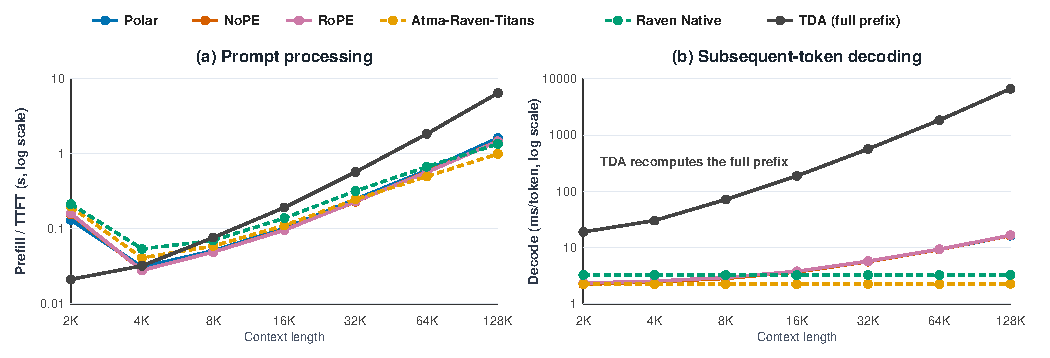
\includegraphics[width=\linewidth]{fig_serving_scaling.pdf}
\caption{Single-sequence serving on one L40S (logarithmic latency axes). Attention models use cached decoding and Raven uses recurrent state; TDA recomputes the full prefix at each token. Prompt measurements are prefill latency for the cached backends and TTFT for TDA. Backend differences preclude an architecture-only speed comparison.}
\label{fig:serving_scaling}
\end{figure}

\begin{table}[h]
\centering
\small
\resizebox{\linewidth}{!}{%
\begin{tabular}{llrrrr}
\toprule
\textbf{Group} & \textbf{Model} & \textbf{Base mean} & \textbf{128K prompt} & \textbf{Decode} & \textbf{Train MFU} \\
& & (\%) & (s) & (ms/token) & (\%, 2K) \\
\midrule
Matched & NoPE & 45.1 & 1.47 & 16.4 & 42.77 \\
Matched & Polar & 43.3 & 1.62 & 16.3 & 40.44 \\
Matched & RoPE & 44.6 & 1.47 & 16.5 & 42.45 \\
AdamW & Atma-Raven-Titans & 43.1 & 1.00 & 2.27 & 30.92 \\
AdamW & Raven Native & 43.0 & 1.36 & 3.27 & 21.53 \\
\midrule
AdamW/direct & TDA hybrid & 40.6 & 6.46 & 6668.5 & 38.64 \\
\bottomrule
\end{tabular}}
\caption{Short-context and systems trade-offs on one L40S, one sequence and one timing sample. TDA uses full-prefix recomputation (TTFT); other rows use cached/recurrent serving (prefill). Backend differences preclude an architecture-only speed comparison. Memory complexity and allocation accounting are detailed in Appendix~\ref{appendix:systems}.}
\label{table:quality_systems_summary}
\end{table}

Table~\ref{table:base_tasks_breakdown} gives the exact per-task controls shown in main-text Figure~\ref{fig:short_context_controls}. Figure~\ref{fig:serving_scaling} shows the serving-length trend, and Table~\ref{table:quality_systems_summary} summarizes the quality--systems trade-off.

\FloatBarrier
\section{Systems Implementation and Optimization Breakdown}
\label{appendix:systems}

The inference stack uses separate kernels for full-context prefill, paged autoregressive decode, and recurrent-state updates. Table~\ref{table:kernel_breakdown} distinguishes what each optimization changes. In particular, streaming removes quadratic score storage but not quadratic prefill arithmetic, while the recurrent Raven path changes the state representation itself and therefore has different scaling.

\begin{table}[!ht]
\centering
\small
\begin{tabular}{p{0.20\linewidth}p{0.34\linewidth}p{0.34\linewidth}}
\toprule
\textbf{Path} & \textbf{Optimization} & \textbf{Operational effect} \\
\midrule
Polar prefill & Block-streamed $K,V$ tiles with online $(M,L,Q_2,S)$ accumulation & Avoids materializing $T\times T$ scores; retains full-context $O(T^2)$ arithmetic. \\
Polar decode & Paged KV-cache kernel grouping the four query heads that share each KV head & Reuses KV loads across the GQA group; decode remains $O(T)$ in cache length. \\
Gated-delta step & Fused in-place decay, prediction, delta write, and readout & Avoids materializing per-step intermediate states and preserves $O(1)$ recurrent state size. \\
Ragged prefill & Packed prompts with grouped compatible tile shapes & Reduces padding work on heterogeneous prompt batches. \\
Compiler boundary & Recurrent scan and custom kernels exposed as opaque operations & Prevents compiler graph breaks around the stateful update while retaining explicit numerical tests. \\
\bottomrule
\end{tabular}
\caption{Implementation-level optimization breakdown. Complexity statements describe the sequence-mixing path and exclude shared MLP and embedding costs.}
\label{table:kernel_breakdown}
\end{table}

\paragraph{Memory accounting.}
Engine allocation includes weights, runtime buffers, and any preallocated KV pool. The attention runner sizes its pool against a 90\% device-memory budget, whereas Raven allocates recurrent state without a KV pool. The roughly 39.4 GiB attention values therefore reflect the configured engine's allocation policy and do not measure the minimum memory required for one 128K sequence. With four global layers, two KV heads, head dimension 128, and BF16 storage, the occupied key/value tensors for that sequence require $2\times4\times131{,}072\times2\times128\times2$ bytes, or 0.5 GiB, before weights, activations, recurrent state, and other buffers. This is an analytical KV-size calculation, not a new peak-memory measurement. The recurrent-state and KV-length complexity comparison remains separate from these allocated-pool measurements.

\begin{landscape}
\subsection{Single-sequence scaling}
TDA has no cached decoder in this repository. Table~\ref{table:serving_detailed_matrix} measures the exact forward path with full-prefix recomputation at each generated token, under protocol \texttt{direct-full-recompute-v1}. Each shape receives a full warmup; loading and tokenization are excluded, and CUDA synchronization brackets timing. At 128K, TTFT is 6.464\,s and subsequent decoding is 0.150 tokens/s, with 5.98/11.00\,GiB peak allocated/reserved memory. These are executable-backend measurements, not a bound on optimized TDA performance or a like-for-like comparison with paged serving.

Table~\ref{table:serving_detailed_matrix} gives the underlying single-sequence measurements. On one NVIDIA L40S, attention decode increases from approximately 2.3 ms/token at 2K to 16.3--16.5 ms/token at 128K because every step reads a longer KV cache. The recurrent models remain nearly flat because they update fixed-size state. Prefill is less monotonic at short lengths because launch overhead and kernel occupancy dominate before the matrix operations reach their efficient regime. These timings use batch size 1, 32 generated tokens, and one recorded timing sample per cell. They are descriptive measurements, not confidence intervals.
\begingroup
\small
\setlength{\tabcolsep}{4pt}
\begin{longtable}{llrrrrrrr}
\caption{Detailed prefill and decode scaling from 2K to 128K tokens on one NVIDIA L40S GPU (batch size 1, 32 generated tokens).}\label{table:serving_detailed_matrix}\\
\toprule
\textbf{Model} & \textbf{Metric} & \textbf{2K} & \textbf{4K} & \textbf{8K} & \textbf{16K} & \textbf{32K} & \textbf{64K} & \textbf{128K} \\
\midrule
\endfirsthead
\caption[]{Detailed prefill and decode scaling (continued).}\\
\toprule
\textbf{Model} & \textbf{Metric} & \textbf{2K} & \textbf{4K} & \textbf{8K} & \textbf{16K} & \textbf{32K} & \textbf{64K} & \textbf{128K} \\
\midrule
\endhead
\midrule
\multicolumn{9}{r}{Continued on next page}\\
\endfoot
\bottomrule
\endlastfoot
Polar & Prefill latency (s) & 0.131 & 0.031 & 0.051 & 0.101 & 0.248 & 0.601 & 1.619 \\
& Prefill throughput (tok/s) & 15,640 & 133,884 & 160,145 & 161,551 & 132,091 & 109,050 & 80,959 \\
& Decode latency (ms/tok) & 2.27 & 2.49 & 2.88 & 3.70 & 5.66 & 9.22 & 16.30 \\
& Decode throughput (tok/s) & 441.2 & 402.3 & 346.6 & 270.1 & 176.8 & 108.5 & 61.3 \\
\midrule
NoPE & Prefill latency (s) & 0.157 & 0.028 & 0.049 & 0.097 & 0.230 & 0.576 & 1.473 \\
& Prefill throughput (tok/s) & 13,070 & 146,568 & 166,504 & 168,510 & 142,319 & 113,810 & 89,013 \\
& Decode latency (ms/tok) & 2.22 & 2.45 & 2.83 & 3.68 & 5.62 & 9.22 & 16.40 \\
& Decode throughput (tok/s) & 450.1 & 408.8 & 353.0 & 271.7 & 177.8 & 108.4 & 61.0 \\
\midrule
RoPE & Prefill latency (s) & 0.160 & 0.028 & 0.049 & 0.096 & 0.232 & 0.566 & 1.472 \\
& Prefill throughput (tok/s) & 12,761 & 147,089 & 168,287 & 170,936 & 141,249 & 115,786 & 89,015 \\
& Decode latency (ms/tok) & 2.34 & 2.53 & 2.95 & 3.79 & 5.73 & 9.33 & 16.51 \\
& Decode throughput (tok/s) & 427.4 & 395.3 & 338.7 & 263.7 & 174.5 & 107.2 & 60.6 \\
\midrule
Atma-Raven-Titans & Prefill latency (s) & 0.198 & 0.041 & 0.059 & 0.111 & 0.247 & 0.499 & 0.999 \\
& Prefill throughput (tok/s) & 10,334 & 100,989 & 137,903 & 147,434 & 132,916 & 131,464 & 131,195 \\
& Decode latency (ms/tok) & 2.24 & 2.25 & 2.24 & 2.24 & 2.26 & 2.25 & 2.27 \\
& Decode throughput (tok/s) & 446.6 & 445.1 & 446.0 & 447.1 & 442.6 & 444.8 & 440.3 \\
\midrule
Raven Native & Prefill latency (s) & 0.214 & 0.054 & 0.070 & 0.139 & 0.320 & 0.672 & 1.357 \\
& Prefill throughput (tok/s) & 9,558 & 75,738 & 116,378 & 117,605 & 102,354 & 97,527 & 96,559 \\
& Decode latency (ms/tok) & 3.26 & 3.25 & 3.24 & 3.24 & 3.25 & 3.25 & 3.27 \\
& Decode throughput (tok/s) & 306.4 & 307.5 & 308.2 & 308.3 & 307.6 & 307.5 & 306.1 \\
\midrule
\multicolumn{9}{l}{\textit{Direct full-prefix recomputation (different backend)}} \\
TDA hybrid & Prefill latency (s) & 0.021 & 0.032 & 0.077 & 0.193 & 0.572 & 1.843 & 6.464 \\
& Prefill throughput (tok/s) & 96,599 & 127,449 & 107,079 & 85,065 & 57,271 & 35,553 & 20,276 \\
& Decode latency (ms/tok) & 18.97 & 30.26 & 71.44 & 187.59 & 565.26 & 1837.32 & 6668.50 \\
& Decode throughput (tok/s) & 52.7 & 33.0 & 14.0 & 5.3 & 1.8 & 0.5 & 0.1 \\
\end{longtable}
\endgroup
\end{landscape}

\subsection{Production-framework stress comparison}
To test whether the custom kernels introduce an obvious systems bottleneck at a larger shape, we configured ATMA's inference engine with a 9.2B-parameter stress shape and compared it with vLLM 0.25.0 serving Qwen3.5-9B on the same L40S in BF16~\citep{kwon2023vllm}. The models are not weight- or architecture-matched, so Table~\ref{table:vllm_comparison_matrix} is a backend stress comparison rather than a model-quality or universal serving claim. ATMA trails on short homogeneous prefill, is similar on long heterogeneous prefill, and leads the recorded high-batch decode cells.

\begin{table}[!ht]
\centering
\small
\setlength{\tabcolsep}{4pt}
\resizebox{\linewidth}{!}{%
\begin{tabular}{llrrr}
\toprule
\textbf{Phase} & \textbf{Batch/workload} & \textbf{ATMA engine} & \textbf{vLLM/Qwen3.5-9B} & \textbf{Ratio} \\
\midrule
Prefill & Homogeneous $B=8,T=512$ (4,096 tok) & 11,947 tok/s & 12,772 tok/s & 0.94$\times$ \\
& Heterogeneous short-heavy (816 tok) & 5,752 tok/s & 8,002 tok/s & 0.72$\times$ \\
& Heterogeneous mixed (4,384 tok) & 12,779 tok/s & 11,996 tok/s & 1.07$\times$ \\
& Heterogeneous long-tail (8,192 tok) & 12,251 tok/s & 11,721 tok/s & 1.05$\times$ \\
\midrule
Decode, context 512 & Batch 128 & 2,939 tok/s & 2,247 tok/s & 1.31$\times$ \\
& Batch 256 & 4,501 tok/s & 2,921 tok/s & 1.54$\times$ \\
& Batch 512 & 5,919 tok/s & 2,558 tok/s & 2.31$\times$ \\
& Heterogeneous $B=128$ (context 64--1536) & 2,950 tok/s & 2,403 tok/s & 1.23$\times$ \\
\bottomrule
\end{tabular}}
\caption{Recorded systems-scale throughput for ATMA's 9.2B stress shape and vLLM 0.25.0 serving Qwen3.5-9B on one L40S (BF16, greedy sampling). Ratio is ATMA/vLLM.}
\label{table:vllm_comparison_matrix}
\end{table}

\section{Retention-Horizon Diagnostic}
\label{appendix:retention_audit}

This section records the post-hoc sequence from parameter inspection to a multi-clamp sweep and broad benchmark re-evaluation. It analyzes released checkpoints rather than a new trained architecture. The primary checkpoint comparisons in Section 5 show untouched models together with explicitly marked inference-only caps. Every cap below is opt-in, applied only at inference, and removed after each condition.

The diagnostic follows three systematic stages:
\begin{enumerate}
  \item \textbf{Parameter-only operating point inspection:} Identifying unusually large learned retention gate biases ($b_\gamma$) without running the model.
  \item \textbf{Causal multi-clamping sweep:} Evaluating multiple clamp values (local percentiles \texttt{p90}, \texttt{p99} and absolute half-life ceilings \texttt{hl:256}, \texttt{hl:512}) across sequence lengths 2K--256K on clean text loss and needle retrieval.
  \item \textbf{Independent benchmark re-evaluation:} Re-benchmarking the selected intervention across short-context downstream tasks, retrieval (synthetic and FinePDFs real-text haystacks, passkey and NIAH), fixed-target long-document likelihood (FinePDFs, PG-19, Proof-Pile), and BABILong reasoning.
\end{enumerate}

Figure~\ref{fig:main_results} shows the complete primary before/after curves alongside the untouched reference models.

\subsection{Parameter-only operating points}
The memory gate has one learned row per query/memory head, rather than one scalar per attention KV head. For each row we decompose the logit as
\begin{equation}
 z_{\gamma,t}=W_\gamma x_t+b_\gamma,\qquad
 \gamma_0=\sigma(b_\gamma),\qquad
 H_{1/2}(\gamma_0)=\frac{\log(1/2)}{\log\gamma_0}.
\end{equation}
Here $x=0$ defines a reproducible learned operating point. It is not the empirical mean runtime gate: every reported outlier has a nonzero $W_\gamma$ row, so activations can shorten or lengthen its instantaneous horizon.

Table~\ref{table:gamma_parameters_full} reports the parameter operating points across all base checkpoints. The promoted NoPE and Polar checkpoints trained on L40S contain isolated Block 2 heads with learned half-lives of $21.01$M and $3.07$M tokens. RoPE has a maximum $H_{1/2}$ of 682.2 tokens, while Atma-Raven-Titans ranges from $30.5$ to $41.4$ tokens. We therefore do not cap Atma-Raven-Titans.

Scanning the separately fine-tuned BABILong checkpoints gives 20.86M tokens for NoPE, 3.05M for Polar, and 680 for RoPE. The outlier therefore remains nearly unchanged after adaptation. Each BABILong cap is still selected from the final fine-tuned checkpoint rather than copied from the base model.

For TDA hybrid, a parameter scan covers all 64 memory layer-heads in both base and adapted checkpoints. For $\gamma_0=\sigma(b_\gamma+\mathrm{mem\_gamma\_bias})$, the maximum zero-input half-life is 36.74379 tokens in both checkpoints (zero-based block 6, head 7), with $\gamma_0=0.981312483$. No head exceeds 256 tokens at zero input. This scan does not exhibit the extreme parameter-only outlier seen in NoPE. However, token-dependent gates can exceed their zero-input values: the maximum head's input-weight row has nonzero norm (approximately 1.273). The scan neither bounds runtime retention nor explains retrieval decay. No capped TDA benchmark was run, and no claim that the cap is inert follows from this diagnostic.

\subsection{Paired multi-clamp sweep}
For a target maximum half-life $H_{\max}$, the diagnostic clips the final activation-conditioned gate logit,
\begin{equation}
 z'_{\gamma,t}=\min\!\left(z_{\gamma,t},\operatorname{logit}(2^{-1/H_{\max}})\right),\qquad
 \gamma'_t=\sigma(z'_{\gamma,t}).
\end{equation}
For \texttt{hl:256}, $H_{\max}=256 \implies \gamma'_t\leq0.997296$. Only the single layer/head with the largest parameter-only $b_\gamma$ is targeted. This upper bound leaves smaller token-conditioned gates unchanged, modifies neither checkpoint tensors nor attention, and is removed after the condition.

Table~\ref{table:gamma_sweep_full} reports the complete paired sweep across conditions (\texttt{baseline}, \texttt{p90}, \texttt{p99}, \texttt{hl:256}, \texttt{hl:512}) and lengths (2K, 16K, 64K, 256K) within a single process sharing model instance, documents, and seeds:
\begin{itemize}
  \item \textbf{Why \texttt{hl:256} is selected:} It gives the largest reduction in 256K needle cross-entropy, from $12.20$ to $6.05$ nats on NoPE and from $2.39$ to $1.71$ nats on Polar. It also keeps 2K clean-loss drift within the $0.05$-nat guardrail, at $+0.022$ nats on NoPE and $+0.010$ on Polar.
  \item \textbf{Why \texttt{p99} fails on saturated checkpoints:} On NoPE L40S, the 99th-percentile logit ($13.46$) still gives a half-life of about 484k tokens. At 256K, clean loss remains at $12.09$ nats and needle cross-entropy at $12.15$ nats.
  \item \textbf{Why RoPE is an empirical negative control:} RoPE has no comparable outlier. Capping it at \texttt{hl:256} gives no retrieval benefit at 256K ($0.0\%$ accuracy) and reduces short-context needle accuracy from $82.5\%$ to $50.0\%$. The intervention is therefore not a general benchmark boost.
\end{itemize}

\subsection{Independent benchmark re-evaluation}
After the pilot sweep, we evaluate the capped promoted checkpoints on all eight short-context downstream tasks, the full synthetic and FinePDFs retrieval matrix, dataset-level long-document likelihood, and BABILong QA1--QA10. Base-model and BABILong-fine-tuned checkpoints are pinned to their archived Hugging Face revisions. Direct checkpoint-exact scoring is used throughout. All 15 model--suite jobs completed without an out-of-memory failure.

Tables~\ref{table:gamma_parameters_full}--\ref{table:gamma_longdoc_dataset_breakdown} report the full numerical arrays:
\begin{itemize}
  \item \textbf{Downstream Controls (Table~\ref{table:gamma_downstream_full}):} Unweighted 2K task means change by at most $0.06$ points across all three models, showing small changes in the aggregate downstream mean; this does not imply preservation of every short-context retrieval metric.
  \item \textbf{Retrieval curves (Tables~\ref{table:gamma_retrieval_token_full}, \ref{table:gamma_retrieval_exact_full}, \ref{table:gamma_haystack_retrieval_full}, \ref{table:gamma_haystack_retrieval_exact_full}):} Polar gains $+12.70$ points in target-token accuracy and $+7.33$ points in exact five-token accuracy at 256K. Its 8K FinePDFs exact accuracy rises from 62.7\% to 91.3\%, and capped exact recall remains nonzero through 128K. NoPE remains at 0.0\% exact real-text retrieval from 16K to 256K, and RoPE remains at 0.0\% at every extrapolation length.
  \item \textbf{BABILong reasoning (Table~\ref{table:gamma_babilong_full}):} The cap raises NoPE to $35$--$57\%$ from 8K to 256K, compared with 39/21/6\% untouched at 8/16/32K and 0\% from 64K onward, and raises Polar from $28\%$ to $42\%$ at 256K. RoPE decreases from $14\%$ to $11\%$.
  \item \textbf{Long-document likelihood (Tables~\ref{table:gamma_bpb_full}, \ref{table:gamma_longdoc_dataset_breakdown}):} At 256K, the cap reduces NoPE BPB from $11.666$ to $1.180$ on FinePDFs, from $4.902$ to $1.224$ on PG-19, and from $7.723$ to $2.382$ on Proof-Pile. Polar's mean degradation drops from $1.26\times$ to $1.03\times$.
\end{itemize}

\input{gamma_re_evaluation_tables.tex}

These results support an isolated near-unit retention gate as a major mediator of NoPE and Polar extrapolation degradation. They motivate testing bounded retention gates during training, but the inference-only intervention does not validate that design.

The complete machine-readable artifacts are under \texttt{gamma\_diagnostics/results/}: \texttt{parameters/gamma\_parameters.json} for the scan, \texttt{all\_clamp\_sweep\_262k.json} for the paired pilot, and \texttt{re\_evaluation/run-summary.json} plus per-suite logs for the full benchmark. The executable protocol and reporting caveats are in \texttt{gamma\_diagnostics/README.md}.

\subsection{Follow-up Evaluation: Adaptation Interaction, Specificity Controls, and Replications}
\label{appendix:pat_feedback}

Following evaluation review feedback, we executed prospective follow-up experiments under \texttt{supplementary/pat\_feedback/} to settle component attribution, test retention limits across continuous pre-training (CPT), and audit numerical operator parity.

\paragraph{Numerical Semantics and Operator Parity (E0).}
Direction-floor evaluation audited the theoretical floor formula $U / \max(\|U\|_2, \epsilon Z)$ against the streaming implementation $U / \max(\|U\|_2, \epsilon)$. In the operational regime where $\|s\|_2 \ge \epsilon$, the two expressions are mathematically identical and agree to $0.0$ error in FP64. Checkpoint probes across 256K context sequences on Stage II and Foveal Polar checkpoints confirmed a 0.0\% floor activation rate. Testing the learned-temperature control $t(n) = 1 + \operatorname{softplus}(\alpha) \log(n)$ with $t=1$ verified exact recovery of ordinary NoPE SDPA and shared parameter gradients with $0.0$ error.

\paragraph{Retention Capping across Adaptation States (E2).}
To establish whether the retention cap's efficacy depends on continuous pre-training, we evaluated eight conditions (2 cores $\times$ 2 adaptation states $\times$ 2 cap conditions) on the frozen 18-document likelihood panel:
\begin{itemize}
  \item \textbf{Original Stage II checkpoints:} Uncapped NoPE exhibits severe degradation beyond 2K, reaching 8.098 BPB at 256K; capping its single outlier head (B2/H5) recovers likelihood to 1.595 BPB ($+6.503$ cap benefit $B$). Primary Polar 256K BPB drops from 1.855 to 1.520 ($+0.334$ cap benefit $B$).
  \item \textbf{Foveal CPT checkpoints:} After 1B tokens of CPT at 32K context, uncapped NoPE already stabilizes at 1.567 BPB at 256K, and capping yields a modest $+0.079$ BPB improvement (1.488 BPB). Foveal Polar uncapped 256K BPB is 1.461, and capped is 1.439 ($+0.021$ cap benefit $B$).
  \item \textbf{Adaptation contrast:} The cap benefit is substantially larger on unadapted models than on adapted ones: $B(\text{original}) - B(\text{foveal}) = +6.424$ in NoPE and $+0.313$ in Polar. Foveal adaptation's modified context exposure and routing dynamics diminish the necessity of a post-hoc retention intervention.
\end{itemize}

\paragraph{Runtime Telemetry (E3).}
Activation-conditioned telemetry confirms that the outlier heads maintain extreme median half-lives ($>3 \times 10^8$ tokens) under live text inputs when uncapped, which are strictly capped to 256 tokens under the \texttt{hl-256} intervention. Write gates ($\beta$) remain moderate ($0.04$--$0.09$ for NoPE, $0.21$--$0.30$ for Polar). In Foveal checkpoints, the parameter-only outlier persists, but surrounding sparse attention insulating the residual stream prevents catastrophic likelihood collapse.

\paragraph{Independent-Document Retrieval Replications (E4).}
Evaluating six untouched checkpoints across 30 independently sampled natural FinePDFs documents (averaging passkey and NIAH across three depths, 8K--64K) confirms Polar's retrieval superiority across initializations:
\begin{itemize}
  \item Primary pair: Polar achieves 36.25\% exact natural-text retrieval versus NoPE's 0.97\% ($+35.28\%$ contrast).
  \item Replication seed 1: Polar achieves 37.92\% versus NoPE's 1.25\% ($+36.67\%$ contrast).
  \item Replication seed 2: Polar achieves 42.22\% versus NoPE's 2.64\% ($+39.58\%$ contrast).
  \item Paired bootstrap: Document-cluster paired bootstrap (10,000 resamples, seed 20270915) confirms an average $+37.18\%$ natural-text retrieval advantage for Polar across seeds.
\end{itemize}

\paragraph{Ceiling Sensitivity and Head Specificity (E5).}
A sweep over cap ceilings ($H \in \{128, 256, 512, 1024\}$) on the six-document diagnostic subset shows that ceilings between 128 and 512 tokens effectively prevent 256K likelihood collapse, with $H=256$ optimal. In contrast, applying $H=256$ to alternative same-layer heads (the second-highest $H_0$ head or a randomly chosen same-layer head) yields $0.0$ likelihood recovery (NoPE 256K BPB remains at $7.53$--$7.62$). The intervention's curative effect is strictly head-specific.

\paragraph{Temperature-Matched Component Attribution (E1).}
To separate the contributions of Polar's direction normalization, null competitor, and learned length temperatures, protocol E1 executes three matched arms across three initialization seeds (20270912, 20270913, 20270914): ordinary \texttt{nope\_memory}, \texttt{temperature\_softmax\_memory} using $\tau(n) = 1 + \operatorname{softplus}(\alpha) \ln(n)$ (introducing exactly 32 learned $\alpha$ parameters matching Polar's per-head temperature parameterization), and full \texttt{polar\_memory}. Each run trains for 1,900 optimizer updates ($996{,}147{,}200$ tokens) on the identical sorted shard order, maintaining byte-identical post-initialization common weights verified by SHA-256 digests across arms. As shown in Table~\ref{table:component_attribution_e1}, Polar strictly outperforms temperature-matched softmax across all three initialization seeds on 8K--64K natural-text exact retrieval: $+30.56\%$ in Triplet 1 (36.25\% vs 5.69\%), $+31.53\%$ in Triplet 2 (44.86\% vs 13.33\%), and $+4.44\%$ in Triplet 3 (48.61\% vs 44.17\%), yielding a mean primary contrast of $+22.18\%$. This confirms that Polar's retrieval superiority cannot be attributed merely to the learned length-temperature family; direction normalization and the null competitor are essential to its long-context fidelity.

\begin{table}[!ht]
\centering
\small
\setlength{\tabcolsep}{5pt}
\begin{tabular}{lcccccc}
\toprule
\textbf{Triplet} & \textbf{Seed} & \textbf{NoPE} & \textbf{Temp-Softmax} & \textbf{Polar} & \textbf{Polar vs Temp} & \textbf{Polar vs NoPE} \\
\midrule
Triplet 1 & 20270912 & 5.69\% & 5.69\% & 36.25\% & \textbf{+30.56\%} & +30.56\% \\
Triplet 2 & 20270913 & 16.67\% & 13.33\% & 44.86\% & \textbf{+31.53\%} & +28.19\% \\
Triplet 3 & 20270914 & 15.42\% & 44.17\% & 48.61\% & \textbf{+4.44\%} & +33.19\% \\
\midrule
\textbf{Mean} & — & \textbf{12.59\%} & \textbf{21.06\%} & \textbf{43.24\%} & \textbf{+22.18\%} & \textbf{+30.65\%} \\
\bottomrule
\end{tabular}
\caption{Component attribution results across three independent initialization triplets (8K--64K mean natural-text exact retrieval on 30 independent documents). Polar consistently outperforms temperature-softmax, establishing an average $+22.18\%$ primary advantage.}
\label{table:component_attribution_e1}
\end{table}

\paragraph{Controlled Serving Repeatability (E6).}
To ensure serving benchmarks are repeatable and eliminate launch-timing artifacts, we conducted 10 timed repetitions per model and context length with strict GPU synchronization on one NVIDIA L40S, with untimed warmups and isolated memory resets:
\begin{itemize}
  \item \textbf{Recurrent and Hybrid Decoders:} Raven Native exhibits strictly length-invariant decode latency of $3.27$--$3.32$\,ms/token ($301$--$305$\,tokens/s) from 2K to 128K context. Atma-Raven-Titans decodes at $2.25$--$2.30$\,ms/token ($434$--$444$\,tokens/s) through 128K context, confirming that fixed-size recurrent state tables isolate decode latency from prefix length.
  \item \textbf{Paged Attention Decoders:} NoPE, RoPE, and Polar exhibit identical short-context decode latencies ($2.20$--$2.31$\,ms/token at 2K), scaling monotonically to $14.81$--$15.51$\,ms/token ($65$--$68$\,tokens/s) at 128K as every decode step traverses the growing KV cache ($7.01$--$7.27$\,GiB peak memory).
  \item \textbf{TDA Upstream Prefill:} Using the official Triton parallel kernel, TDA achieves prefill throughput of $86{,}532$\,tokens/s at 2K, $57{,}005$\,tokens/s at 32K, and $19{,}851$\,tokens/s at 128K ($6.60$\,s TTFT). Autoregressive decode is omitted because upstream Snap Research authors provided no cached incremental decode kernel, and prefix recomputation artificially degrades decode speed.
\end{itemize}

\begin{table}[!ht]
\centering
\small
\setlength{\tabcolsep}{4.5pt}
\begin{tabular}{lcccccc}
\toprule
\textbf{Architecture} & \textbf{2K TTFT} & \textbf{2K Decode} & \textbf{32K TTFT} & \textbf{32K Decode} & \textbf{128K TTFT} & \textbf{128K Decode} \\
\midrule
NoPE & 0.024\,s & 2.20\,ms (454\,t/s) & 0.227\,s & 5.24\,ms (191\,t/s) & 1.487\,s & 14.81\,ms (68\,t/s) \\
Polar & 0.025\,s & 2.27\,ms (440\,t/s) & 0.029\,s & 5.45\,ms (183\,t/s) & 0.065\,s & 15.51\,ms (65\,t/s) \\
RoPE & 0.023\,s & 2.31\,ms (433\,t/s) & 0.231\,s & 5.35\,ms (187\,t/s) & 1.505\,s & 14.96\,ms (67\,t/s) \\
Raven Native & 0.045\,s & 3.27\,ms (305\,t/s) & 0.314\,s & 3.28\,ms (305\,t/s) & 1.333\,s & 3.32\,ms (301\,t/s) \\
Atma-Raven-Titans & 0.029\,s & 2.25\,ms (444\,t/s) & 0.243\,s & 2.25\,ms (444\,t/s) & 0.999\,s & 2.30\,ms (434\,t/s) \\
TDA (Hybrid) & 0.024\,s & \textit{Skipped} & 0.575\,s & \textit{Skipped} & 6.603\,s & \textit{Skipped} \\
\bottomrule
\end{tabular}
\caption{Controlled serving repeatability on one NVIDIA L40S across 10 timed repetitions (batch size 1, 32 generated tokens). TTFT denotes time-to-first-token. TDA decode is omitted due to the absence of an upstream cached decode kernel.}
\label{table:serving_repeatability_e6}
\end{table}

\section{Stress and Environment Diagnostics}
\label{appendix:diagnostics}

\begin{figure}[h]
\centering
\includegraphics[width=\linewidth]{fig_stress_heatmap.pdf}
\caption{Block-wise sampled secant gains for the three matched attention checkpoints over 64 nested FinePDFs documents and 64 perturbation directions per document. Raven Native and Atma-Raven-Titans were not run under this checkpoint-specific probe. The diagnostic localizes changes but does not estimate a global Lipschitz constant.}
\label{fig:appendix_stress_heatmap}
\end{figure}

Figure~\ref{fig:appendix_stress_heatmap} reports the sampled gains. For each block $f_i$, the diagnostic samples
\begin{equation}
G_i=\frac{\lVert f_i(x+\delta x)-f_i(x)\rVert_{\rm rms}}{\lVert\delta x\rVert_{\rm rms}},
\qquad \lVert\delta x\rVert_{\rm rms}=0.02\lVert x\rVert_{\rm rms}.
\end{equation}
The maximum sampled gain is a lower bound on the local operator norm along sampled directions. It is not a tight bound on the block Lipschitz constant. In the observed NoPE collapse, changes first concentrate near blocks 6--7 and later propagate through the residual stream. Polar's sampled gains and activation moments remain comparatively flat through 256K.

\section{Checkpoint-Variability Diagnostic Journey}
\label{appendix:environment}

The variability finding emerged sequentially. Stage I used L4 GPUs, followed by the first 10B NoPE control on an L4. The difference became visible after primary training moved to L40S. Short-context convergence remained close (2.8126 vs 2.8160 nats; approximately 0.12\% difference), while 256K NLL differed (4.07 vs 10.77 nats). Table~\ref{table:environment_diagnostic_journey} records the seven-step diagnostic sequence and the retention-horizon intervention.

\begin{table}[!ht]
\centering
\small
\setlength{\tabcolsep}{4pt}
\begin{tabular}{>{\raggedright\arraybackslash}p{0.20\linewidth}>{\raggedright\arraybackslash}p{0.36\linewidth}>{\raggedright\arraybackslash}p{0.38\linewidth}}
\toprule
\textbf{Step} & \textbf{Observation or intervention} & \textbf{Diagnostic implication} \\
\midrule
1. L4 baseline & Stage I and first 10B NoPE control on L4 (mbs4); 256K NLL was 4.07. & Established baseline extrapolation, but lacked replicated device-class controls. \\
2. L40S transition & Promoted NoPE run on L40S (mbs16); 2K validation matched (2.8126 vs 2.8160), but 256K NLL rose to 10.77. & Showed that the short-context pretraining curves did not predict long-context behavior. \\
3. Evaluation replay & L4 and L40S checkpoints re-evaluated under PyTorch 2.12 and 2.13 with identical metrics. & Excluded evaluation software runtime mismatch as the source. \\
4. Microbatch control & NoPE retrained on L40S with mbs4; 2K validation ended at 2.8128 and 256K NLL at 9.90. & Showed that microbatch size four did not reliably prevent collapse; initialization remained uncontrolled. \\
5. Deterministic fixtures & Synthetic 2K stream fixtures across device classes showed zero gradient or loss divergence. & Confirmed short-context kernel execution consistency; left training trajectory unconstrained. \\
6. Retention parameter inspection & Evaluated learned zero-input operating point $\gamma_0 = \sigma(b_\gamma)$ across all layers and heads. & \textbf{Identified an outlier:} L40S NoPE developed an isolated Block 2 head with $b_\gamma = +13.33$ ($H_{1/2} = 21.01$M tokens), whereas L4 NoPE had max $H_{1/2} = 185.3$ tokens. \\
7. Single-head causal intervention & Installed a reversible inference cap ($H_{\max} = 256$ tok) on the single outlier head and re-evaluated 2K--256K. & \textbf{Tested the mechanism:} Capping the outlier head reduced 256K NLL from 12.00 to 1.14 nats and raised 256K BABILong to 39\%, supporting excessive retention as a mediator of the collapse. \\
\bottomrule
\end{tabular}
\caption{Diagnostic sequence from the initial L4/L40S divergence to the retention-horizon intervention. Steps 1--5 tested evaluation artifacts and showed that reducing microbatch size did not reliably prevent the failure. Steps 6--7 identified the isolated retention-gate outlier and tested its effect.}
\label{table:environment_diagnostic_journey}
\end{table}

This sequence localizes the observed checkpoint failure to one unusually long zero-input retention horizon, and the inference cap reverses much of the measured degradation. It does not establish what training event produced the outlier or whether hardware-level differences contributed to it. All five headline Stage II models were trained in the same L40S environment, providing an internally controlled comparison for those runs.


\end{document}
